% Options for packages loaded elsewhere
\PassOptionsToPackage{unicode}{hyperref}
\PassOptionsToPackage{hyphens}{url}
%
\documentclass[
  english,
  doc,floatsintext]{apa6}
\usepackage{amsmath,amssymb}
\usepackage{lmodern}
\usepackage{ifxetex,ifluatex}
\ifnum 0\ifxetex 1\fi\ifluatex 1\fi=0 % if pdftex
  \usepackage[T1]{fontenc}
  \usepackage[utf8]{inputenc}
  \usepackage{textcomp} % provide euro and other symbols
\else % if luatex or xetex
  \usepackage{unicode-math}
  \defaultfontfeatures{Scale=MatchLowercase}
  \defaultfontfeatures[\rmfamily]{Ligatures=TeX,Scale=1}
\fi
% Use upquote if available, for straight quotes in verbatim environments
\IfFileExists{upquote.sty}{\usepackage{upquote}}{}
\IfFileExists{microtype.sty}{% use microtype if available
  \usepackage[]{microtype}
  \UseMicrotypeSet[protrusion]{basicmath} % disable protrusion for tt fonts
}{}
\makeatletter
\@ifundefined{KOMAClassName}{% if non-KOMA class
  \IfFileExists{parskip.sty}{%
    \usepackage{parskip}
  }{% else
    \setlength{\parindent}{0pt}
    \setlength{\parskip}{6pt plus 2pt minus 1pt}}
}{% if KOMA class
  \KOMAoptions{parskip=half}}
\makeatother
\usepackage{xcolor}
\IfFileExists{xurl.sty}{\usepackage{xurl}}{} % add URL line breaks if available
\IfFileExists{bookmark.sty}{\usepackage{bookmark}}{\usepackage{hyperref}}
\hypersetup{
  pdftitle={DAP Project: Early Biomarkers of Parkinson's Disease Based on Natural Connected Speech},
  pdfauthor={Anja Probst1},
  pdflang={en-EN},
  hidelinks,
  pdfcreator={LaTeX via pandoc}}
\urlstyle{same} % disable monospaced font for URLs
\usepackage{color}
\usepackage{fancyvrb}
\newcommand{\VerbBar}{|}
\newcommand{\VERB}{\Verb[commandchars=\\\{\}]}
\DefineVerbatimEnvironment{Highlighting}{Verbatim}{commandchars=\\\{\}}
% Add ',fontsize=\small' for more characters per line
\usepackage{framed}
\definecolor{shadecolor}{RGB}{248,248,248}
\newenvironment{Shaded}{\begin{snugshade}}{\end{snugshade}}
\newcommand{\AlertTok}[1]{\textcolor[rgb]{0.94,0.16,0.16}{#1}}
\newcommand{\AnnotationTok}[1]{\textcolor[rgb]{0.56,0.35,0.01}{\textbf{\textit{#1}}}}
\newcommand{\AttributeTok}[1]{\textcolor[rgb]{0.77,0.63,0.00}{#1}}
\newcommand{\BaseNTok}[1]{\textcolor[rgb]{0.00,0.00,0.81}{#1}}
\newcommand{\BuiltInTok}[1]{#1}
\newcommand{\CharTok}[1]{\textcolor[rgb]{0.31,0.60,0.02}{#1}}
\newcommand{\CommentTok}[1]{\textcolor[rgb]{0.56,0.35,0.01}{\textit{#1}}}
\newcommand{\CommentVarTok}[1]{\textcolor[rgb]{0.56,0.35,0.01}{\textbf{\textit{#1}}}}
\newcommand{\ConstantTok}[1]{\textcolor[rgb]{0.00,0.00,0.00}{#1}}
\newcommand{\ControlFlowTok}[1]{\textcolor[rgb]{0.13,0.29,0.53}{\textbf{#1}}}
\newcommand{\DataTypeTok}[1]{\textcolor[rgb]{0.13,0.29,0.53}{#1}}
\newcommand{\DecValTok}[1]{\textcolor[rgb]{0.00,0.00,0.81}{#1}}
\newcommand{\DocumentationTok}[1]{\textcolor[rgb]{0.56,0.35,0.01}{\textbf{\textit{#1}}}}
\newcommand{\ErrorTok}[1]{\textcolor[rgb]{0.64,0.00,0.00}{\textbf{#1}}}
\newcommand{\ExtensionTok}[1]{#1}
\newcommand{\FloatTok}[1]{\textcolor[rgb]{0.00,0.00,0.81}{#1}}
\newcommand{\FunctionTok}[1]{\textcolor[rgb]{0.00,0.00,0.00}{#1}}
\newcommand{\ImportTok}[1]{#1}
\newcommand{\InformationTok}[1]{\textcolor[rgb]{0.56,0.35,0.01}{\textbf{\textit{#1}}}}
\newcommand{\KeywordTok}[1]{\textcolor[rgb]{0.13,0.29,0.53}{\textbf{#1}}}
\newcommand{\NormalTok}[1]{#1}
\newcommand{\OperatorTok}[1]{\textcolor[rgb]{0.81,0.36,0.00}{\textbf{#1}}}
\newcommand{\OtherTok}[1]{\textcolor[rgb]{0.56,0.35,0.01}{#1}}
\newcommand{\PreprocessorTok}[1]{\textcolor[rgb]{0.56,0.35,0.01}{\textit{#1}}}
\newcommand{\RegionMarkerTok}[1]{#1}
\newcommand{\SpecialCharTok}[1]{\textcolor[rgb]{0.00,0.00,0.00}{#1}}
\newcommand{\SpecialStringTok}[1]{\textcolor[rgb]{0.31,0.60,0.02}{#1}}
\newcommand{\StringTok}[1]{\textcolor[rgb]{0.31,0.60,0.02}{#1}}
\newcommand{\VariableTok}[1]{\textcolor[rgb]{0.00,0.00,0.00}{#1}}
\newcommand{\VerbatimStringTok}[1]{\textcolor[rgb]{0.31,0.60,0.02}{#1}}
\newcommand{\WarningTok}[1]{\textcolor[rgb]{0.56,0.35,0.01}{\textbf{\textit{#1}}}}
\usepackage{longtable,booktabs,array}
\usepackage{calc} % for calculating minipage widths
% Correct order of tables after \paragraph or \subparagraph
\usepackage{etoolbox}
\makeatletter
\patchcmd\longtable{\par}{\if@noskipsec\mbox{}\fi\par}{}{}
\makeatother
% Allow footnotes in longtable head/foot
\IfFileExists{footnotehyper.sty}{\usepackage{footnotehyper}}{\usepackage{footnote}}
\makesavenoteenv{longtable}
\usepackage{graphicx}
\makeatletter
\def\maxwidth{\ifdim\Gin@nat@width>\linewidth\linewidth\else\Gin@nat@width\fi}
\def\maxheight{\ifdim\Gin@nat@height>\textheight\textheight\else\Gin@nat@height\fi}
\makeatother
% Scale images if necessary, so that they will not overflow the page
% margins by default, and it is still possible to overwrite the defaults
% using explicit options in \includegraphics[width, height, ...]{}
\setkeys{Gin}{width=\maxwidth,height=\maxheight,keepaspectratio}
% Set default figure placement to htbp
\makeatletter
\def\fps@figure{htbp}
\makeatother
\setlength{\emergencystretch}{3em} % prevent overfull lines
\providecommand{\tightlist}{%
  \setlength{\itemsep}{0pt}\setlength{\parskip}{0pt}}
\setcounter{secnumdepth}{-\maxdimen} % remove section numbering
% Make \paragraph and \subparagraph free-standing
\ifx\paragraph\undefined\else
  \let\oldparagraph\paragraph
  \renewcommand{\paragraph}[1]{\oldparagraph{#1}\mbox{}}
\fi
\ifx\subparagraph\undefined\else
  \let\oldsubparagraph\subparagraph
  \renewcommand{\subparagraph}[1]{\oldsubparagraph{#1}\mbox{}}
\fi
% Manuscript styling
\usepackage{upgreek}
\captionsetup{font=singlespacing,justification=justified}

% Table formatting
\usepackage{longtable}
\usepackage{lscape}
% \usepackage[counterclockwise]{rotating}   % Landscape page setup for large tables
\usepackage{multirow}		% Table styling
\usepackage{tabularx}		% Control Column width
\usepackage[flushleft]{threeparttable}	% Allows for three part tables with a specified notes section
\usepackage{threeparttablex}            % Lets threeparttable work with longtable

% Create new environments so endfloat can handle them
% \newenvironment{ltable}
%   {\begin{landscape}\begin{center}\begin{threeparttable}}
%   {\end{threeparttable}\end{center}\end{landscape}}
\newenvironment{lltable}{\begin{landscape}\begin{center}\begin{ThreePartTable}}{\end{ThreePartTable}\end{center}\end{landscape}}

% Enables adjusting longtable caption width to table width
% Solution found at http://golatex.de/longtable-mit-caption-so-breit-wie-die-tabelle-t15767.html
\makeatletter
\newcommand\LastLTentrywidth{1em}
\newlength\longtablewidth
\setlength{\longtablewidth}{1in}
\newcommand{\getlongtablewidth}{\begingroup \ifcsname LT@\roman{LT@tables}\endcsname \global\longtablewidth=0pt \renewcommand{\LT@entry}[2]{\global\advance\longtablewidth by ##2\relax\gdef\LastLTentrywidth{##2}}\@nameuse{LT@\roman{LT@tables}} \fi \endgroup}

% \setlength{\parindent}{0.5in}
% \setlength{\parskip}{0pt plus 0pt minus 0pt}

% Overwrite redefinition of paragraph and subparagraph by the default LaTeX template
% See https://github.com/crsh/papaja/issues/292
\makeatletter
\renewcommand{\paragraph}{\@startsection{paragraph}{4}{\parindent}%
  {0\baselineskip \@plus 0.2ex \@minus 0.2ex}%
  {-1em}%
  {\normalfont\normalsize\bfseries\itshape\typesectitle}}

\renewcommand{\subparagraph}[1]{\@startsection{subparagraph}{5}{1em}%
  {0\baselineskip \@plus 0.2ex \@minus 0.2ex}%
  {-\z@\relax}%
  {\normalfont\normalsize\itshape\hspace{\parindent}{#1}\textit{\addperi}}{\relax}}
\makeatother

% \usepackage{etoolbox}
\makeatletter
\patchcmd{\HyOrg@maketitle}
  {\section{\normalfont\normalsize\abstractname}}
  {\section*{\normalfont\normalsize\abstractname}}
  {}{\typeout{Failed to patch abstract.}}
\patchcmd{\HyOrg@maketitle}
  {\section{\protect\normalfont{\@title}}}
  {\section*{\protect\normalfont{\@title}}}
  {}{\typeout{Failed to patch title.}}
\makeatother

\usepackage{xpatch}
\makeatletter
\xapptocmd\appendix
  {\xapptocmd\section
    {\addcontentsline{toc}{section}{\appendixname\ifoneappendix\else~\theappendix\fi\\: #1}}
    {}{\InnerPatchFailed}%
  }
{}{\PatchFailed}
\usepackage{csquotes}
\usepackage{dcolumn}
\ifxetex
  % Load polyglossia as late as possible: uses bidi with RTL langages (e.g. Hebrew, Arabic)
  \usepackage{polyglossia}
  \setmainlanguage[]{english}
\else
  \usepackage[main=english]{babel}
% get rid of language-specific shorthands (see #6817):
\let\LanguageShortHands\languageshorthands
\def\languageshorthands#1{}
\fi
\ifluatex
  \usepackage{selnolig}  % disable illegal ligatures
\fi
\newlength{\cslhangindent}
\setlength{\cslhangindent}{1.5em}
\newlength{\csllabelwidth}
\setlength{\csllabelwidth}{3em}
\newenvironment{CSLReferences}[2] % #1 hanging-ident, #2 entry spacing
 {% don't indent paragraphs
  \setlength{\parindent}{0pt}
  % turn on hanging indent if param 1 is 1
  \ifodd #1 \everypar{\setlength{\hangindent}{\cslhangindent}}\ignorespaces\fi
  % set entry spacing
  \ifnum #2 > 0
  \setlength{\parskip}{#2\baselineskip}
  \fi
 }%
 {}
\usepackage{calc}
\newcommand{\CSLBlock}[1]{#1\hfill\break}
\newcommand{\CSLLeftMargin}[1]{\parbox[t]{\csllabelwidth}{#1}}
\newcommand{\CSLRightInline}[1]{\parbox[t]{\linewidth - \csllabelwidth}{#1}\break}
\newcommand{\CSLIndent}[1]{\hspace{\cslhangindent}#1}

\title{DAP Project: Early Biomarkers of Parkinson's Disease Based on Natural Connected Speech}
\author{Anja Probst\textsuperscript{1}}
\date{}


\shorttitle{DAP Project}

\authornote{

The authors made the following contributions. Anja Probst: Conceptualization, Writing - Original Draft Preparation, Writing - Review \& Editing.

Correspondence concerning this article should be addressed to Anja Probst, 24 rue du Général-Dufour, 1211 Genève 4. E-mail: \href{mailto:anja.probst@etu.unige.ch}{\nolinkurl{anja.probst@etu.unige.ch}}

}

\affiliation{\vspace{0.5cm}\textsuperscript{1} University of Geneva}

\abstract{
Parkinson's Disease is a degenerative disorder of the nervous system that
globally affects more than 6 million people.
While the most well-recognized symptoms of the disease are motor-related, such
as shaking and instability, a further group of symptoms, which is only partially motor-related
and occurs in a majority of patients, are speech-altering symptoms.
While the disease is well-recognizable at a later stage, it is exceptionally hard to diagnose
and differentiate in its early stages and appropriate treatment is often delayed.
In 2017, Hlavnička et al.~have published a study suggesting that automated analysis of connected
speech can reveal early biomarkers even in subjects with REM sleep behaviour disorder, who are at
high risk of developing Parkinson's disease. In this project I analyse the data set published by
the authors that contains experimental evaluation of healthy controls, subjects with REM
sleep behaviour disorder, and subjects with Parkinson's Disease. While the constraints
of this project limit the scope of analysis, I could show that it is possible to create binomial
and mutlinomial models that reach specificity in detecting Parkinson's of up to 75\% in healthy
controls and 71\% in a mix of healthy controls and REM sleep behaviour disorder subjects.
}



\begin{document}
\maketitle

\clearpage

\hypertarget{introduction}{%
\section{Introduction}\label{introduction}}

\hypertarget{context-of-the-project}{%
\subsection{Context of the Project}\label{context-of-the-project}}

Patients with the neurodegenerative disease Parkinson's have numerous symptoms ranging from cognitive
impairments to motor symptoms. Those symptoms may appear relatively late in the disease when the
neurodegeneration has already widely spread in different areas of the brain (mainly Basal Ganglia).
Main symptoms of PD are motor dysfunctions including abnormalities in the production and sound of
speech of such patients (up to 90\%). These abnormalities in speech and voice are called hypokinetic
dysarthria which is characterized by a decreased quality of the speech, where the voice, sound formation
as well as the articulation is impaired. As I mentioned before, often motor impairments are detected
relatively late in the disease. To improve diagnostics and to detect the disease in a much earlier stage,
the detection of biomarkers related to neurodegeneration could lead to a better prognosis and therapy of PD.
(Dashtipour, Tafreshi, Lee, \& Crawley, 2018; Vos et al., 2016)

Therefore, the investigation of prodromal speech changes could be an appropriate and suitable approach.
To investigate this approach, an automated speech monitoring system was developed, that uses a
segmentation method for the precise estimation of voiced and unvoiced segments of speech, respirations,
and pauses. Further proposed was a set of acoustic speech features based on the segmentation algorithm
applicable to connected speech, allowing the description of complex vocal disturbances due to neurodegeneration
including respiratory deficits, dysphonia, imprecise articulation, and dysrhythmia.

In this data analysis project, the main focus is to explore, if there are any speech patterns that
support the usage of an automated speech monitoring system to detect prodromal parkinsonian
neurodegeneration based on natural connected speech.

Therefore my main hypothesis is, that there are speech related variables, that can detect Parkinson's disease
in individuals, and distinguish between individuals with Parkinson's disease and individuals with REM sleep
behaviour disorder despite them exhibiting similar speech related symptoms.

The data, which is the basis of this project, was gathered by Hlavnička et al. (2017), and has the following composition:
130 subjects were tested. 30 subjects with early, untreated Parkinson's disease (PD) where the disease
is already manifested. 50 subjects with REM sleep behaviour disorder (RBD), which is a disease where
its relatively likely to develop PD in a later phase. As a control group, 50 healthy subjects (HD) were included.

\hypertarget{manual-variable-selection}{%
\subsection{Manual Variable Selection}\label{manual-variable-selection}}

Due to the constraints of this project, I reduced the data set from originally 62 variables to the best fitting 7.
As I am looking specifically into the aspect of speech, and to evaluate if speech is a good predictor for PD,
I chose speech related variables that were assessed empirically and were reported to have the most significant differences
between healthy controls and subjects with early stages of Parkinson's Disease.
Note that patient group will be extracted from the variable Participant\_code.
The resulting data set is summarized in Table \ref{tab:summarize-data-frame}

\begin{Shaded}
\begin{Highlighting}[]
\NormalTok{cols.to.keep }\OtherTok{\textless{}{-}} \FunctionTok{c}\NormalTok{(}
    \StringTok{"Participant\_code"}\NormalTok{, }\StringTok{"Age"}\NormalTok{, }\StringTok{"Gender"}\NormalTok{, }\StringTok{"Rate\_of\_speech\_timing"}\NormalTok{,}
    \StringTok{"Rate\_of\_speech\_timing.1"}\NormalTok{, }\StringTok{"Duration\_of\_pause\_intervals"}\NormalTok{,}
    \StringTok{"Duration\_of\_pause\_intervals.1"}
\NormalTok{)}

\CommentTok{\# Above columns will be renamed to}
\NormalTok{rename.cols.to }\OtherTok{\textless{}{-}} \FunctionTok{c}\NormalTok{(}
    \StringTok{"Participant\_code"}\NormalTok{, }\StringTok{"Age"}\NormalTok{, }\StringTok{"Gender"}\NormalTok{, }\StringTok{"Reading.Timing"}\NormalTok{,}
    \StringTok{"Monologue.Timing"}\NormalTok{, }\StringTok{"Reading.Duration"}\NormalTok{,}
    \StringTok{"Monologue.Duration"}
\NormalTok{)}

\NormalTok{csv.path }\OtherTok{\textless{}{-}} \StringTok{"BiomarkersPD.csv"}
\NormalTok{df }\OtherTok{\textless{}{-}} \FunctionTok{read.csv}\NormalTok{(csv.path, }\AttributeTok{sep =} \StringTok{","}\NormalTok{, }\AttributeTok{header =} \ConstantTok{TRUE}\NormalTok{)}

\CommentTok{\# Only keep required columns and rename them}
\NormalTok{df }\OtherTok{\textless{}{-}}\NormalTok{ df[cols.to.keep]}
\FunctionTok{colnames}\NormalTok{(df) }\OtherTok{\textless{}{-}}\NormalTok{ rename.cols.to}

\CommentTok{\# Replace "{-}" with NA}
\NormalTok{df[df }\SpecialCharTok{==} \StringTok{"{-}"}\NormalTok{] }\OtherTok{\textless{}{-}} \ConstantTok{NA}

\CommentTok{\# Get groups from participant codes by replacing numerical values}
\NormalTok{df}\SpecialCharTok{$}\NormalTok{Group }\OtherTok{\textless{}{-}} \FunctionTok{gsub}\NormalTok{(}\StringTok{"[[:digit:]]+"}\NormalTok{, }\StringTok{""}\NormalTok{, df}\SpecialCharTok{$}\NormalTok{Participant\_code)}

\CommentTok{\# Participant codes no longer required, remove}
\NormalTok{df }\OtherTok{\textless{}{-}} \FunctionTok{subset}\NormalTok{(df, }\AttributeTok{select =} \SpecialCharTok{{-}}\FunctionTok{c}\NormalTok{(Participant\_code))}

\CommentTok{\# Convert columns to factors}
\NormalTok{col.names }\OtherTok{\textless{}{-}} \FunctionTok{c}\NormalTok{(}\StringTok{"Group"}\NormalTok{, }\StringTok{"Gender"}\NormalTok{)}
\NormalTok{df[col.names] }\OtherTok{\textless{}{-}} \FunctionTok{lapply}\NormalTok{(df[col.names], as.factor)}
\end{Highlighting}
\end{Shaded}

\hypertarget{data-description}{%
\subsection{Data Description}\label{data-description}}

For each sample in this data set (\(n=130\)), there is the following information:

\begin{itemize}
\tightlist
\item
  Demographic information:

  \begin{itemize}
  \tightlist
  \item
    Age (years)
  \item
    Gender (M for male, F for female)
  \end{itemize}
\item
  Speech examination - Speaking task of reading passage: speakers read a standardized, phonetically-balanced text of 80 words twice

  \begin{itemize}
  \tightlist
  \item
    Duration\_Of\_Pause\_Intervals\_Reading: Duration of pause intervals (DPI) describes the quality of speech timing, as pauses can be heavily influenced by the ability to properly initiate speech, it is measured in miliseconds (ms)
  \item
    Rate\_Of\_Speech\_Timing\_Reading: Rate of speech time (RST) includes voiced, unvoiced and pause intervals, it is measured in intervals per minute (-/min)
  \end{itemize}
\item
  Speech examination - Speaking task of monologue: participants were instructed to provide monologue about their interests, job, family or current activities for approximately 90 seconds

  \begin{itemize}
  \tightlist
  \item
    Duration\_Of\_Pause\_Intervals\_Monologue: Duration of pause intervals (DPI) describes the quality of speech timing, as pauses can be heavily influenced by the ability to properly initiate speech, it is measured in milliseconds (ms)
  \item
    Rate\_Of\_Speech\_Timing\_Monologue: Rate of speech time (RST) includes voiced, unvoiced and pause intervals, it is measured in intervals per minute (-/min)
  \end{itemize}
\item
  Group: based on Participant Code

  \begin{itemize}
  \tightlist
  \item
    PD: subjects with Parkinson's disease
  \item
    RBD: subjects with REM sleep behaviour disorder
  \item
    HC: healthy controls
  \end{itemize}
\end{itemize}

\begin{table}[!htbp] \centering \renewcommand*{\arraystretch}{1.1}\caption{Summary of the Data Set used in this Analysis}\label{tab:summarize-data-frame}\resizebox{\textwidth}{!}{
\begin{tabular}{lrrrrrrr}
\hline
\hline
Variable & N & Mean & Std. Dev. & Min & Pctl. 25 & Pctl. 75 & Max \\ 
\hline
Age & 130 & 64.331 & 10.134 & 34 & 58.25 & 72 & 83 \\ 
Gender & 130 &  &  &  &  &  &  \\ 
... F & 27 & 20.8\% &  &  &  &  &  \\ 
... M & 103 & 79.2\% &  &  &  &  &  \\ 
Reading.Timing & 130 & 327.277 & 47.385 & 140 & 297.25 & 358.75 & 457 \\ 
Monologue.Timing & 130 & 288.338 & 52.892 & 112 & 258 & 328.75 & 412 \\ 
Reading.Duration & 130 & 166.646 & 46.488 & 96 & 138.25 & 185 & 388 \\ 
Monologue.Duration & 130 & 229.069 & 79.697 & 117 & 177 & 263.25 & 611 \\ 
Group & 130 &  &  &  &  &  &  \\ 
... HC & 50 & 38.5\% &  &  &  &  &  \\ 
... PD & 30 & 23.1\% &  &  &  &  &  \\ 
... RBD & 50 & 38.5\% &  &  &  &  & \\ 
\hline
\hline
\end{tabular}
}
\end{table}

\begin{verbatim}
'data.frame':   130 obs. of  7 variables:
$ Age : int 58 68 68 75 61 ...
$ Gender : Factor w/ 2 levels "F","M": 1 1 2 2 2 ...
$ Reading.Timing : int 354 340 211 140 269 ...
$ Monologue.Timing : int 333 285 247 112 230 ...
$ Reading.Duration : int 146 173 377 360 211 ...
$ Monologue.Duration: int 158 295 280 397 206 ...
$ Group : Factor w/ 3 levels "HC","PD","RBD": 2 2 2 2 2 ...
\end{verbatim}

\clearpage

\hypertarget{data-pre-processing}{%
\section{Data Pre-Processing}\label{data-pre-processing}}

As an initial step, I created boxplots to check the distribution of the numerical data per group
in detail (Figure \ref{fig:boxplots-and-correlations}).
At first glance, parts of the data show skewed distributions, as the mean (shown as a orange point)
differs substantially in many cases. This might prompt data transformations such as the \(log\)-transform.
Additionally, within each variable, the distributions between the groups were assessed for significant differences.
Here, the data showed significant differences between healthy controls (HC) and Parkinson's (PD) and REM sleep
behaviour disorder subjects (RBD), but no significant differences between PD and RBD. Based on this, I decided
to split the data anlysis part into two sections: (1) Creating a logistic regression model using \texttt{glm} to
discriminate between the two groups HC and PD and (2) creating a multinomial regression model which discriminates
between all three groups (HC, PD, and RBD). There are imbalances in the factors Group and Gender, however, given that
the researchers which created the data did not identify this as an issue, I will not subsample the data set to make
it balanced.

\begin{figure}

{\centering 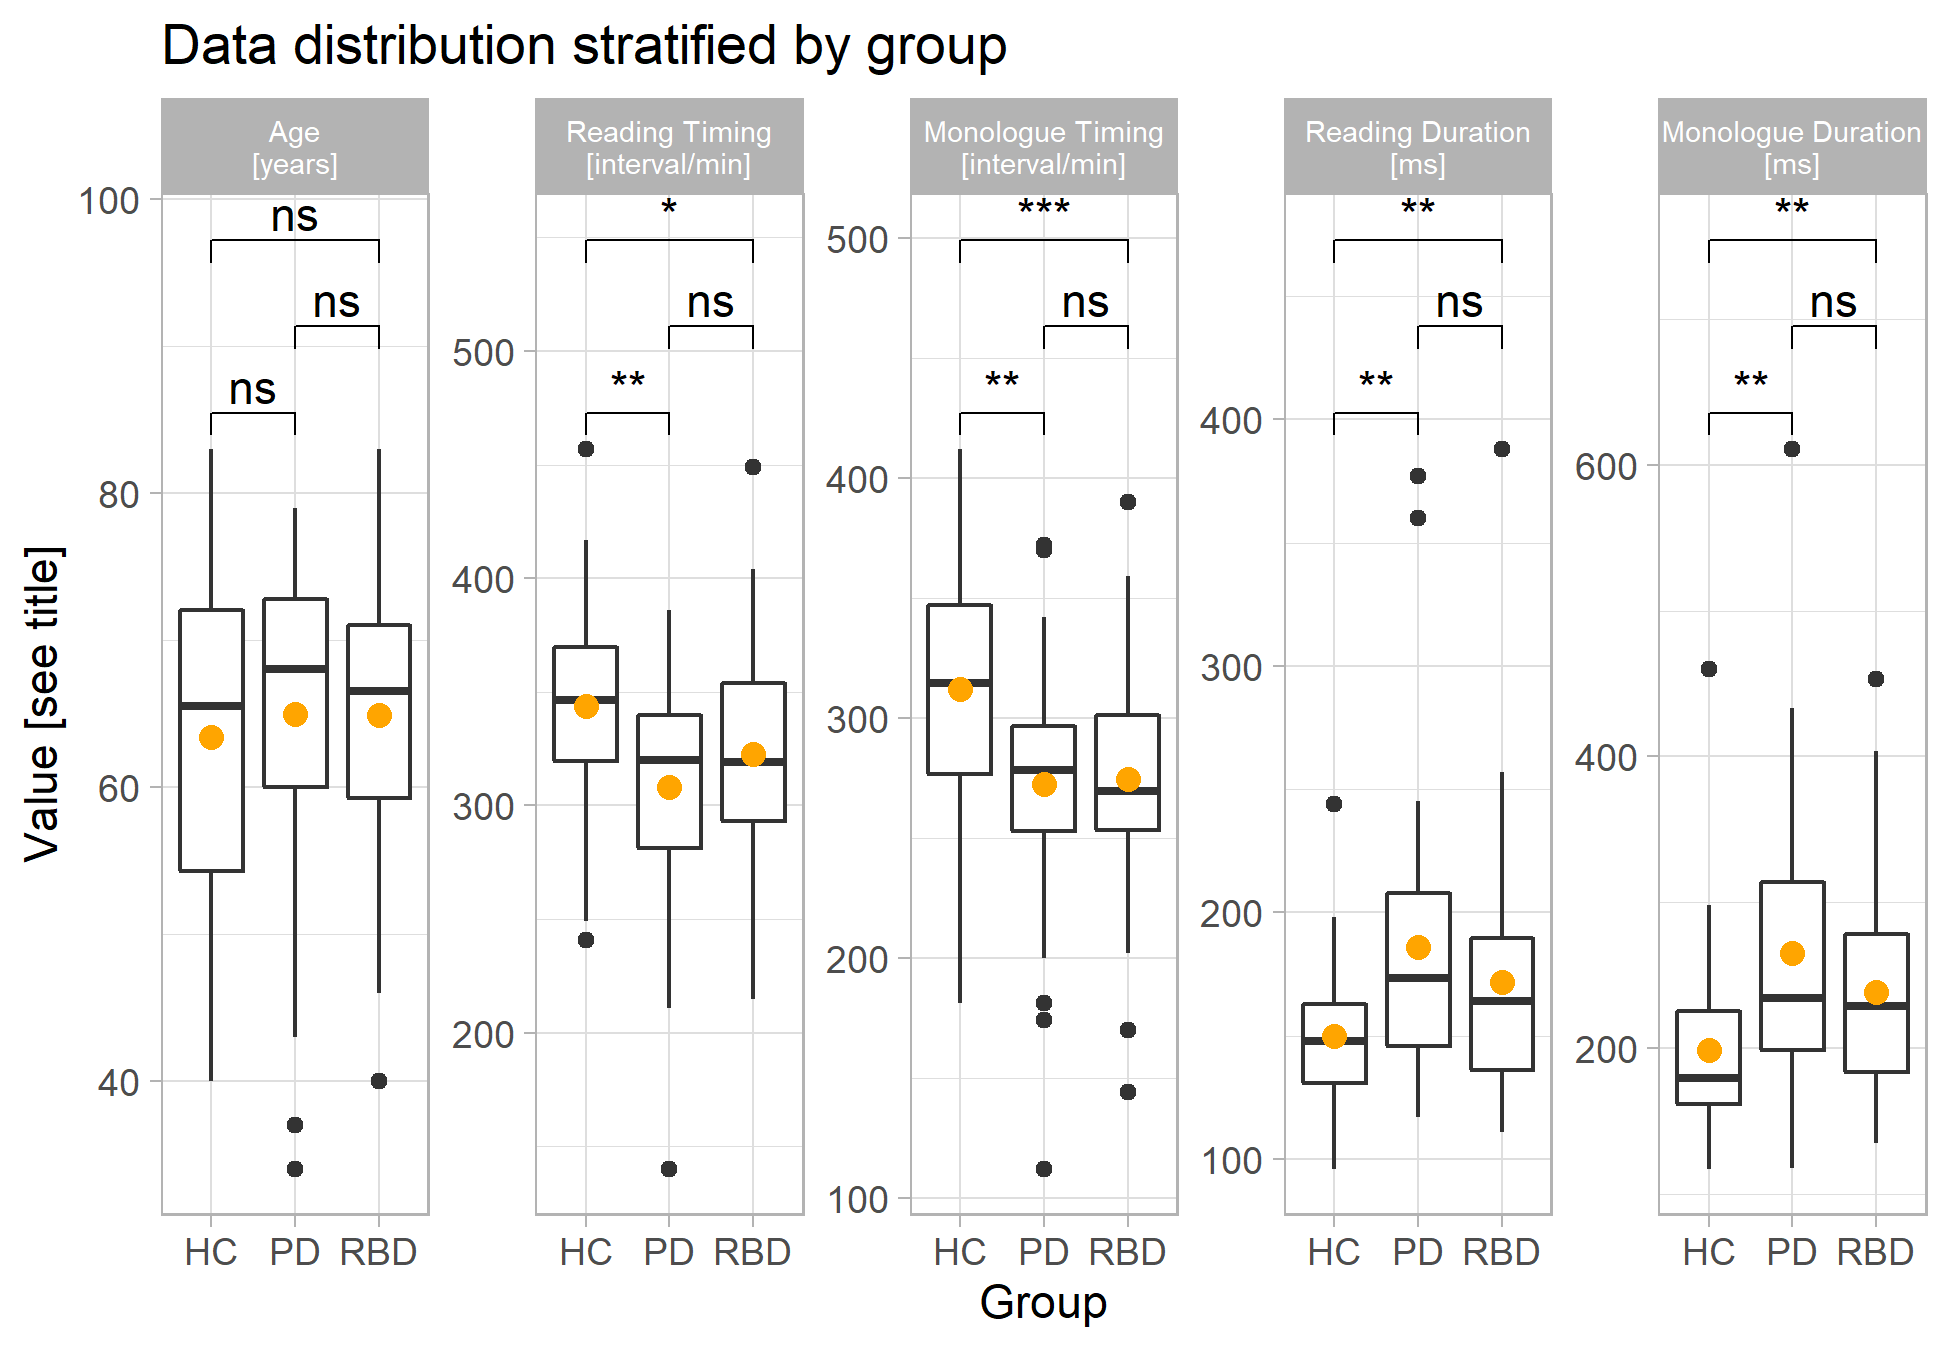
\includegraphics{dap_report_anja_probst_files/figure-latex/boxplots-and-correlations-1} 

}

\caption{Distributions of data within variables and between groups. Some of the data shows skewed distributions (mean is represented by orange point), especially within the variable Age. While there is significant difference (t-Test) between healthy controls (HC) and subjects with Parkinson's disease (PD) as well as REM sleep behaviour disorder (RBD), there are no significant differences between PD and RBD}\label{fig:boxplots-and-correlations}
\end{figure}

Based on visual inspection of the boxplots (Figure \ref{fig:boxplots-and-correlations}),
I chose to remove outliers as shown below.

\begin{Shaded}
\begin{Highlighting}[]
\NormalTok{df.len.before.outlier.removal }\OtherTok{\textless{}{-}} \FunctionTok{nrow}\NormalTok{(df)}
\NormalTok{df }\OtherTok{\textless{}{-}}\NormalTok{ df[df}\SpecialCharTok{$}\NormalTok{Monologue.Duration }\SpecialCharTok{\textless{}} \DecValTok{600}\NormalTok{, ]}
\NormalTok{df }\OtherTok{\textless{}{-}}\NormalTok{ df[df}\SpecialCharTok{$}\NormalTok{Reading.Duration }\SpecialCharTok{\textless{}} \DecValTok{300}\NormalTok{, ]}
\NormalTok{df }\OtherTok{\textless{}{-}}\NormalTok{ df[(df}\SpecialCharTok{$}\NormalTok{Group }\SpecialCharTok{!=} \StringTok{"HC"} \SpecialCharTok{|}\NormalTok{ df}\SpecialCharTok{$}\NormalTok{Monologue.Duration }\SpecialCharTok{\textless{}} \DecValTok{450}\NormalTok{), ]}
\NormalTok{df }\OtherTok{\textless{}{-}}\NormalTok{ df[(df}\SpecialCharTok{$}\NormalTok{Age }\SpecialCharTok{\textgreater{}} \DecValTok{40}\NormalTok{), ]}
\NormalTok{df.len.after.outlier.removal }\OtherTok{\textless{}{-}} \FunctionTok{nrow}\NormalTok{(df)}
\end{Highlighting}
\end{Shaded}

The outlier removel process reduced the size of the data set by 9
from 130 to 121. To further assess the
distributions, which upon visual inspection of the median and mean values in
Figure \ref{fig:boxplots-and-correlations}, \texttt{ggpairs} was run to created by-group density
plots (Figure \ref{fig:correlate-ggpairs-plot}).

\begin{figure}

{\centering 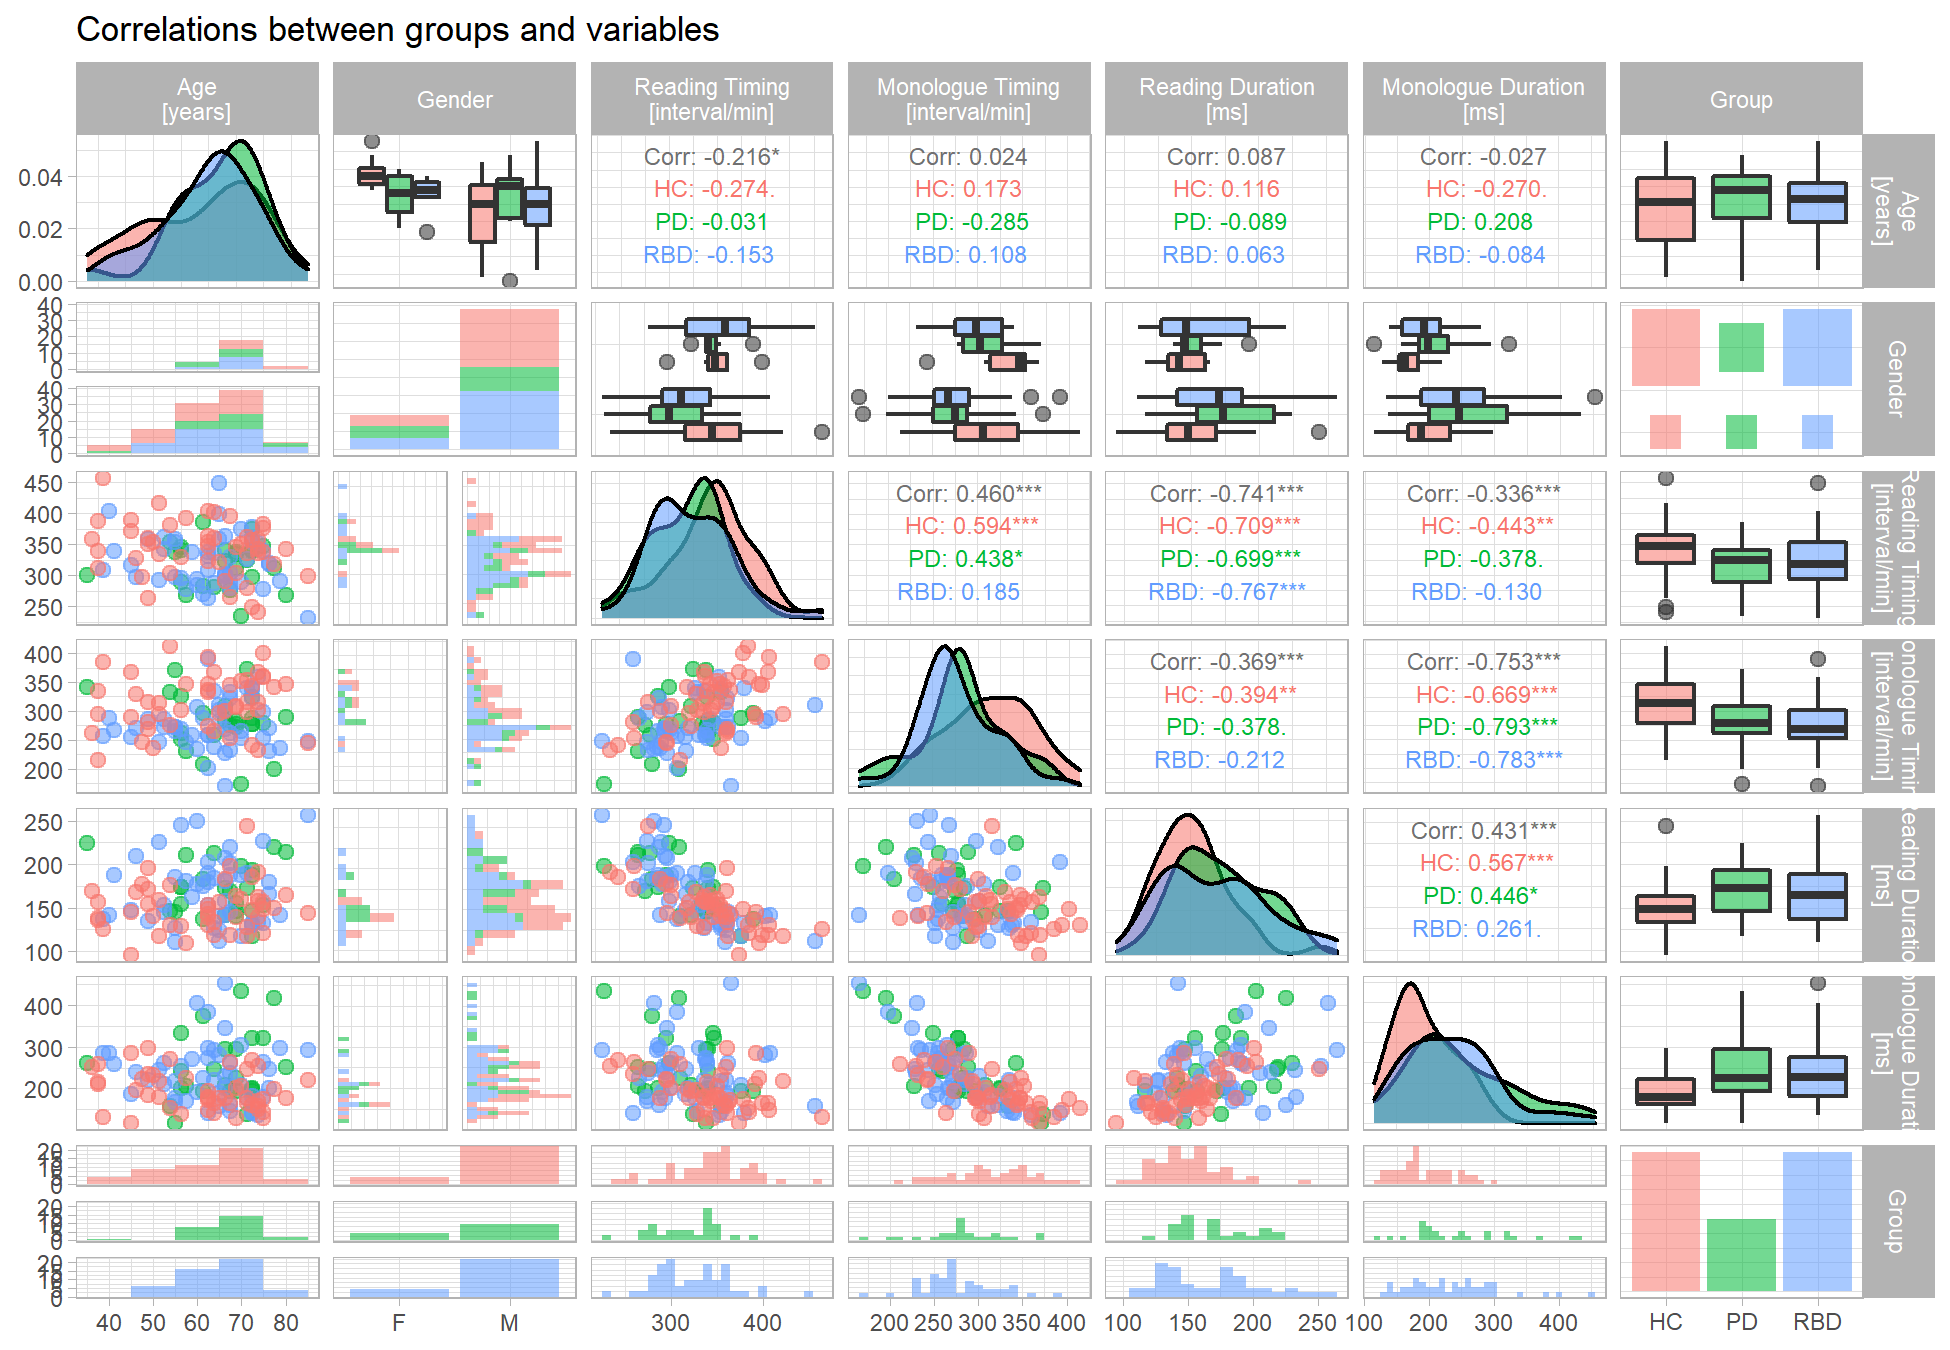
\includegraphics{dap_report_anja_probst_files/figure-latex/correlate-ggpairs-plot-1} 

}

\caption{Plot based on ggpairs, colored by the response variable Group. The empirically collected speech data shows strong correlations (both positive and negative). In addition the density plots show the skewed distributions that were already seen in the boxplots.}\label{fig:correlate-ggpairs-plot}
\end{figure}

Observing Figure \ref{fig:correlate-ggpairs-plot}, the skewness, especially that
of variables Age and Monologue Distribution, becomes apparent. To quantify the deviation from normality,
I tested each distribution for normality using the Shapiro-Wilk normality test. The results shown in
Table \ref{tab:normality-tests} highlight violations of the assumption of normality for both per group
and combinded distributions. For healthy controls (HC) and Parkionson's disease (PD) subjects,
a normal distribution can be assumed for all variables (Reading Time, Monologue Time, Reading Duration,
and Monologue Duration) except Age. For REM sleep behaviour disorder (RBD) subjects normality can
be assumed for variables Age, Reading Timing, and Monologue Timing. In the combined data (Comb.),
only the variables Reading Timing and Monologue Timing can be assumed to be distributed normally.
The observed right and left skewed distributions could be transformed to normal distributions using, for
example, a \(log\)-transform. However, this would lead to a change in distributions for all subgroups,
which do not necessary follow the same (skewed) distribution, as the transform would have to be applied
to all observations of a variable. In addition, such non-linear transformations would greatly hinder the
interpretability of the model. Thus, I chose not to transform the data as part of the data pre-processing.
In a next step, the data is standardized as it contains variables that correlate but have different scales.

\begin{Shaded}
\begin{Highlighting}[]
\NormalTok{df}\SpecialCharTok{$}\NormalTok{Age }\OtherTok{\textless{}{-}} \FunctionTok{c}\NormalTok{(}\FunctionTok{scale}\NormalTok{(df}\SpecialCharTok{$}\NormalTok{Age))}
\NormalTok{df}\SpecialCharTok{$}\NormalTok{Reading.Timing }\OtherTok{\textless{}{-}} \FunctionTok{c}\NormalTok{(}\FunctionTok{scale}\NormalTok{(df}\SpecialCharTok{$}\NormalTok{Reading.Timing))}
\NormalTok{df}\SpecialCharTok{$}\NormalTok{Reading.Duration }\OtherTok{\textless{}{-}} \FunctionTok{c}\NormalTok{(}\FunctionTok{scale}\NormalTok{(df}\SpecialCharTok{$}\NormalTok{Reading.Duration))}
\NormalTok{df}\SpecialCharTok{$}\NormalTok{Monologue.Timing }\OtherTok{\textless{}{-}} \FunctionTok{c}\NormalTok{(}\FunctionTok{scale}\NormalTok{(df}\SpecialCharTok{$}\NormalTok{Monologue.Timing))}
\NormalTok{df}\SpecialCharTok{$}\NormalTok{Monologue.Duration }\OtherTok{\textless{}{-}} \FunctionTok{c}\NormalTok{(}\FunctionTok{scale}\NormalTok{(df}\SpecialCharTok{$}\NormalTok{Monologue.Duration))}
\end{Highlighting}
\end{Shaded}

The data is scaled using the R-function \texttt{scale}, which substracts the variable mean from each observation
and divides the result by the standard deviation of the variable.

\begin{table}[tbp]

\begin{center}
\begin{threeparttable}

\caption{\label{tab:normality-tests}Results of the Shapiro-Wilk test. p-Values are shown in parentheses.
    For healthy controls (HC) and Parkionson's disease (PD) subjects, a normal distribution
    can be assumed for all variables except Age. For REM sleep behaviour disorder
    (RBD) subjects can be assumed for variables Age, Reading Timing, and Monologue Timing.
    In the ungrouped data (Comb.), only the variables Rading Timing and Monologue Timing
    can be assumed to be distributed normally.}

\small{

\begin{tabular}{llllll}
\toprule
Group & \multicolumn{1}{c}{Age} & \multicolumn{1}{c}{Read..Timing} & \multicolumn{1}{c}{Mono..Timing} & \multicolumn{1}{c}{Read..Duration} & \multicolumn{1}{c}{Mono..Duration}\\
\midrule
HC & 0.943 (0.021) & 0.984 (0.733) & 0.984 (0.764) & 0.961 (0.109) & 0.962 (0.117)\\
PD & 0.913 (0.036) & 0.964 (0.501) & 0.964 (0.489) & 0.946 (0.206) & 0.932 (0.098)\\
RBD & 0.972 (0.313) & 0.969 (0.229) & 0.972 (0.299) & 0.948 (0.034) & 0.939 (0.014)\\
Comb. & 0.958 (0.001) & 0.989 (0.456) & 0.99 (0.564) & 0.962 (0.002) & 0.93 (9e-06)\\
\bottomrule
\end{tabular}

}

\end{threeparttable}
\end{center}

\end{table}

\clearpage

\hypertarget{data-analysis}{%
\section{Data Analysis}\label{data-analysis}}

\hypertarget{logistic-regression}{%
\subsection{Logistic Regression}\label{logistic-regression}}

As stated previously, I have seen that there are no significant differences between the groups PD and RBD (Figure \ref{fig:boxplots-and-correlations}).
Based on this observation, I will limit my initial investigation to creating a logistic regression model predicting
between the groups HC and PD. Indeed, the paper from which the data was extracted explicitly
discusses the hard problem of differentiating PD from RBD, which might very well be impossible with
generalised linear models. I will revisit this problem in the section Multinomial Regression.

As a first step, a subset is created that does not contain any observations from the group RBD.

\begin{Shaded}
\begin{Highlighting}[]
\NormalTok{df.binom }\OtherTok{\textless{}{-}} \FunctionTok{data.frame}\NormalTok{(df[df}\SpecialCharTok{$}\NormalTok{Group }\SpecialCharTok{!=} \StringTok{"RBD"}\NormalTok{, ])}
\NormalTok{df.binom}\SpecialCharTok{$}\NormalTok{Group }\OtherTok{\textless{}{-}} \FunctionTok{droplevels}\NormalTok{(df.binom}\SpecialCharTok{$}\NormalTok{Group)}
\NormalTok{df.binom}\SpecialCharTok{$}\NormalTok{Group }\OtherTok{\textless{}{-}} \FunctionTok{relevel}\NormalTok{(df.binom}\SpecialCharTok{$}\NormalTok{Group, }\AttributeTok{ref =} \StringTok{"PD"}\NormalTok{)}
\end{Highlighting}
\end{Shaded}

\hypertarget{initial-model}{%
\subsubsection{Initial Model}\label{initial-model}}

Based on this subset, I first create simple logistic regression models with one response variable
for each of the selected variables (Figure \ref{fig:simple-logistic-regression}). For simplicity
they were created using the \texttt{ggplot2} function \texttt{stat\_smooth}. As can be seen by visual inspection
of the data points (red), none of the predictors is sufficient to predict the response variable
(Group) on its own, given the respective overlap between the two groups.

\begin{figure}

{\centering 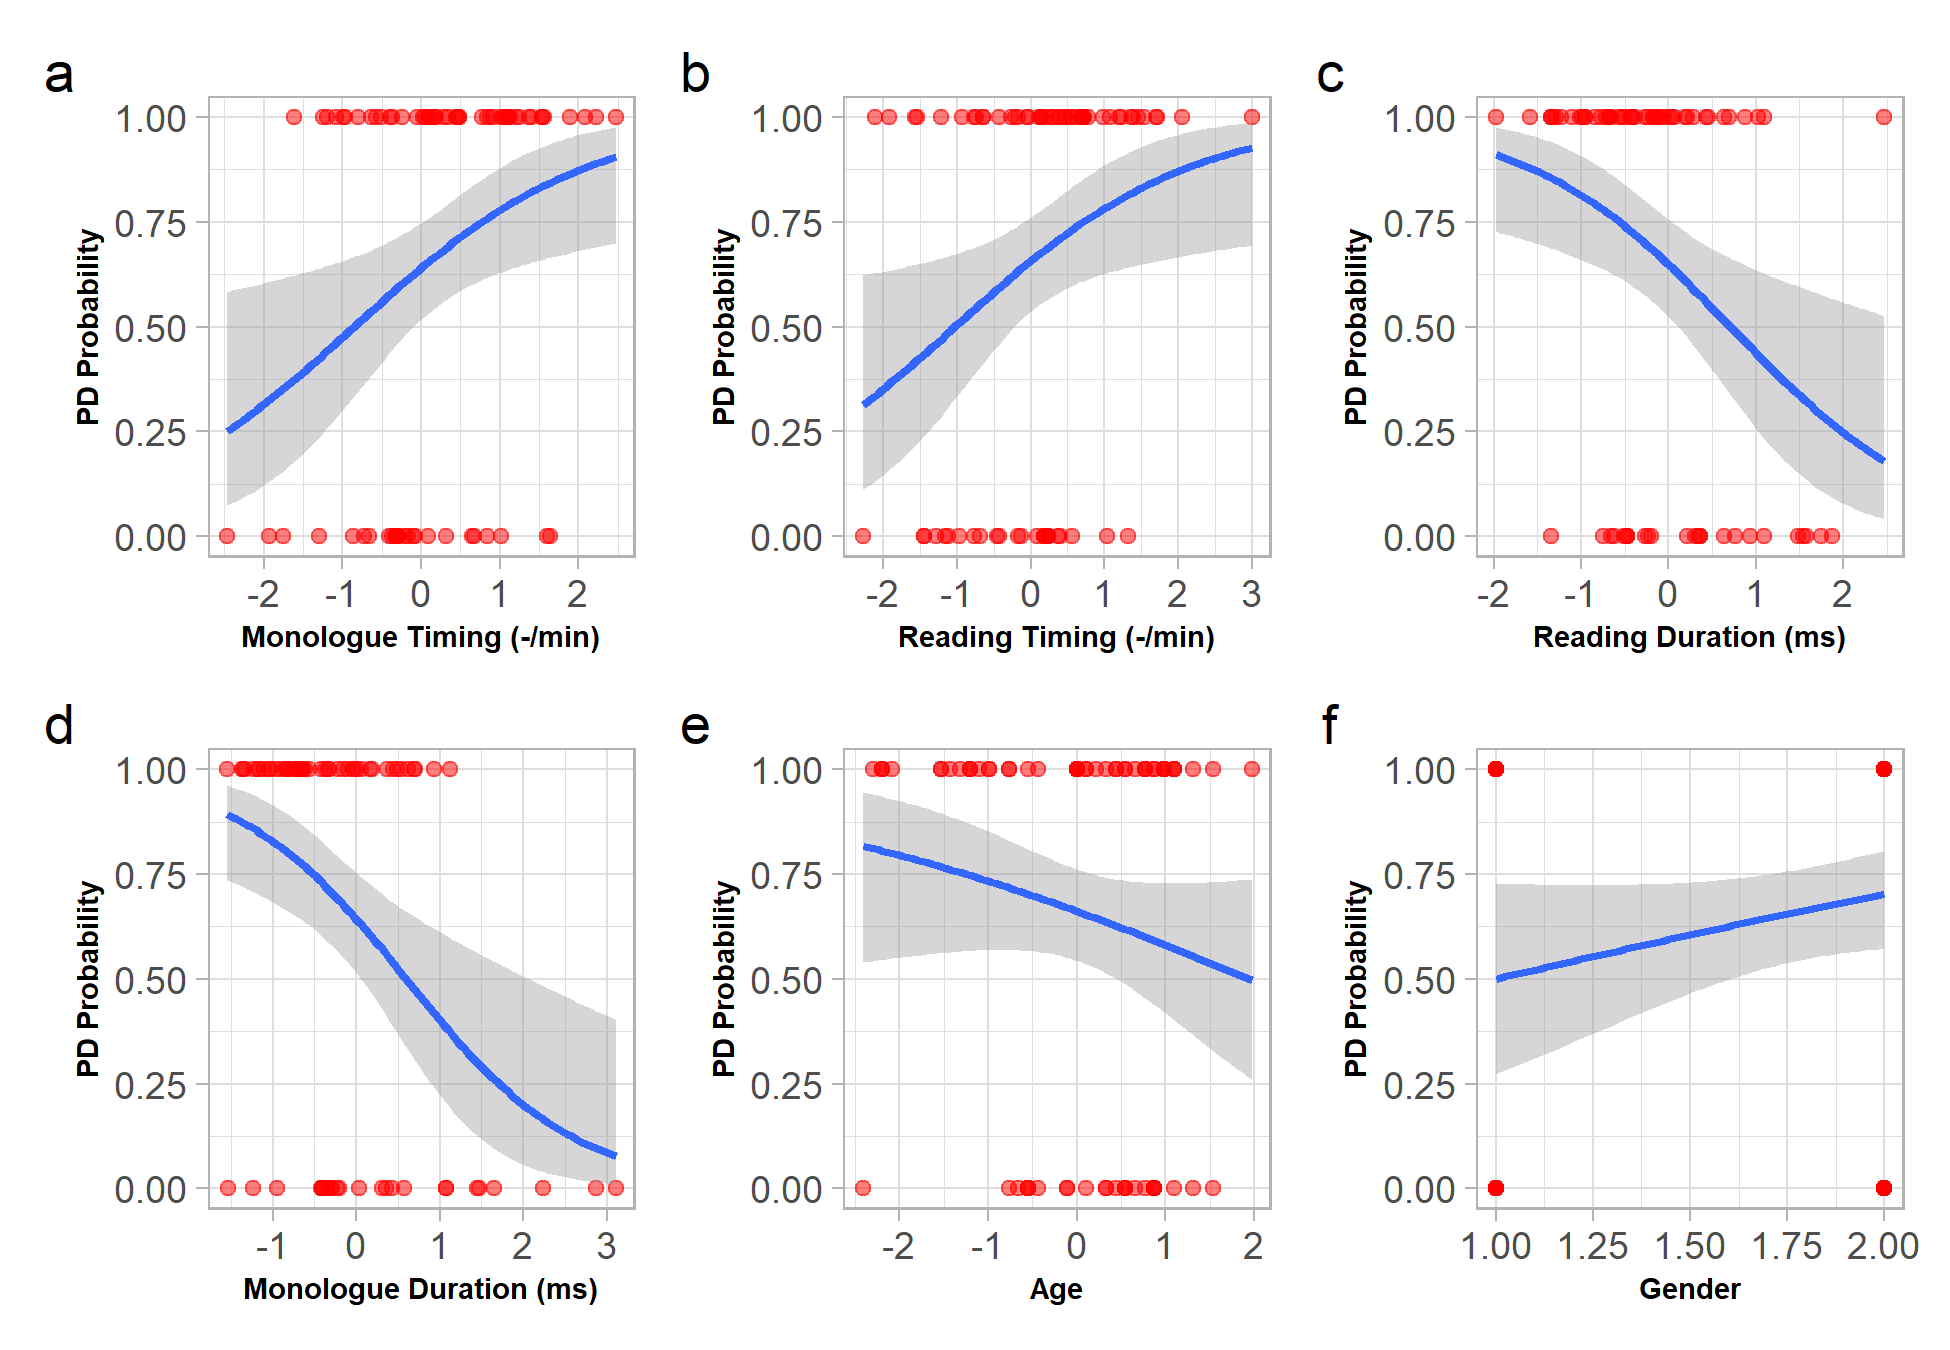
\includegraphics{dap_report_anja_probst_files/figure-latex/simple-logistic-regression-1} 

}

\caption{Simple logistic regression models with one predictor each. The y-axis is the model probability to belong to the group Parkinson's disease (PD). Observations are shown as red points, the blue curve is based on model predictions. For variables a to d, there is a clear sigmoid curve, while variables e, and of course f, which is a factor, do not show such a curve.}\label{fig:simple-logistic-regression}
\end{figure}

Given that a single predictor is clearly not sufficient, a series of multiple logistic regression models
have to be built and evaluated. As I would have to test 64 models (all possible combinations plus
intercept only) to be certain to have found the best one, I instead chose to use the automated model
selection function \texttt{dredge} from the R package \texttt{MuMIn}. Starting from the global binomial model
\texttt{Group\ \textasciitilde{}\ .} as an input, \texttt{dredge} enumerates all possible models and evaluates them based on their AIC.
This is an alternative to manually checking a series of models by starting at the full model and then
removing variables based on AIC and ANOVA comparisons. This manual approach is used in the selection of
the model for the multinomial regression described in the section Multinomial Regression.

\begin{Shaded}
\begin{Highlighting}[]
\NormalTok{m.binom.full }\OtherTok{\textless{}{-}} \FunctionTok{glm}\NormalTok{(}
    \AttributeTok{data =}\NormalTok{ df.binom, Group }\SpecialCharTok{\textasciitilde{}}\NormalTok{ .,}
    \AttributeTok{family =}\NormalTok{ binomial,}
    \AttributeTok{na.action =} \StringTok{"na.fail"}
\NormalTok{)}

\FunctionTok{nrow}\NormalTok{(df.binom[df.binom}\SpecialCharTok{$}\NormalTok{Group }\SpecialCharTok{==} \StringTok{"PD"}\NormalTok{, ])}

\NormalTok{d }\OtherTok{\textless{}{-}} \FunctionTok{dredge}\NormalTok{(m.binom.full, }\AttributeTok{rank =} \StringTok{"AIC"}\NormalTok{)}
\NormalTok{m.binom.no.interactions }\OtherTok{\textless{}{-}} \FunctionTok{get.models}\NormalTok{(d, }\DecValTok{1}\NormalTok{)[[}\DecValTok{1}\NormalTok{]]}
\end{Highlighting}
\end{Shaded}

The results of the model chosen as the best by \texttt{dredge} is \texttt{Group\ \textasciitilde{}\ Gender\ +\ Monologue.Duration\ +\ Reading.Duration},
The model output is shown in Table \ref{tab:model-comparison} (1). As the data was scaled, the constant, or intercept,
coefficient estimate of -0.68 is the logarithmic odds (logits) of a subject having Parkinson's disease, when all other
variables are the average. This is influenced by the number of samples for each of the groups (\(n_{HC}=48\), \$n\_\{PD\}=25).
Using the formula \(p=\frac{exp(coeff)}{1+exp(coeff)}\), which converts the logit to a probability of a subject with all
average measurements has a probability of \(p=\frac{exp(-0.68)}{1+exp(-0.68)}=0.336\) of being predicted to have Parkinson's.
Looking at the coefficients of the model variables Gender, Monolgue Duration, and
Reading Duration, they have effects of different strength in the model. Male gender has a relatively
large, positive effect, meaning that, the probability to be predicted having Parkinson's increases to
\(p=\frac{exp(-0.68 + 1.678)}{1+exp(-0.68 + 1.678)}=0.73\) for men while the other variables stay constant.
This is in line with research that shows that men suffer
more often from Parkinson's (Wooten, Currie, Bovbjerg, Lee, \& Patrie, 2004). As for the two numerical variables Monolgue
Duration and Reading Duration their coefficients of -0.926 and -0.576, respectively, represent
the change in logarithmic odds, as predicted by the model, if their respective value is increased by 1. Here it is
important to remember that the data was scaled according to standard deviation. According to the assessment of the model,
only the coefficients of Gender and Monologue Duration are significant, where the null-hypothesis is that there is no
effect of the inclusion of the variable in the model. The model is evaluated against the following models in the section
Model Comparison and Analysis.

\hypertarget{interactions}{%
\subsubsection{Interactions}\label{interactions}}

Importantly, the automated model selection using \texttt{dredge} did not consider interactions between the predictors.
Given the relatively strong correlation between the speech-related variables, it would be interesting to see
whether a model taking in account the interactions between variables would perform better. In the Appendix, the section
Logistic Regression with Intereactions contains a series of model outputs, in which I tested the inclusion of different
interaction terms. I started with the assumption, that all the measured variables would cause interaction effects
within the model and started reducing the inclusion of interactions from there, finding the model
\texttt{Group\ \textasciitilde{}\ Age\ *\ Gender\ +\ Reading.Timing\ *\ Monologue.Timing\ +\ Reading.Duration\ *\ Monologue.Duration} to have the lowest
AIC and log likelihood (see Appendix Logistic Regression with Intereactions).

\begin{Shaded}
\begin{Highlighting}[]
\NormalTok{m.binom.interactions }\OtherTok{\textless{}{-}} \FunctionTok{glm}\NormalTok{(}
    \AttributeTok{data =}\NormalTok{ df.binom, Group }\SpecialCharTok{\textasciitilde{}}\NormalTok{ Age }\SpecialCharTok{*}\NormalTok{ Gender }\SpecialCharTok{+}\NormalTok{ Reading.Timing }\SpecialCharTok{*}
\NormalTok{        Monologue.Timing }\SpecialCharTok{+}\NormalTok{ Reading.Duration }\SpecialCharTok{*}\NormalTok{ Monologue.Duration,}
    \AttributeTok{family =}\NormalTok{ binomial,}
    \AttributeTok{na.action =} \StringTok{"na.fail"}
\NormalTok{)}
\end{Highlighting}
\end{Shaded}

Coefficients and performance values of this model are found in Table \ref{tab:model-comparison} (2). The interaction
terms are shown in the format variable1:variable2, for example, Reading.Timing:Monologue.Timing with a coefficient of
0.869, which means that when Monologue.Timing increases by 1, 0.869 is added to the logarithmic odds of Reading.Timing
and vice versa.

\hypertarget{pca}{%
\subsubsection{PCA}\label{pca}}

As there has been significant correlation between the predictors in the ggpairs plot
as well as some extreme changes in coefficients when adding additional variables,
there exists the strong possbility of collinearity negatively affecting the models. Indeed,
I observed high variance inflation factors on many predictors in the model with interactions, as
shown in Table \ref{tab:vif}. This warrants an attempt at solving the potential collinearity issue.

\begin{longtable}[]{@{}
  >{\raggedright\arraybackslash}p{(\columnwidth - 2\tabcolsep) * \real{0.53}}
  >{\raggedright\arraybackslash}p{(\columnwidth - 2\tabcolsep) * \real{0.17}}@{}}
\caption{\label{tab:vif} Variance inflation factors (vif) for the model containing
interaction terms (m.binom.interactions).}\tabularnewline
\toprule
Term & VIF Value \\
\midrule
\endfirsthead
\toprule
Term & VIF Value \\
\midrule
\endhead
Age & 32.93 \\
Gender & 4.236 \\
Reading.Timing & 3.538 \\
Monologue.Timing & 2.664 \\
Reading.Duration & 2.42 \\
Monologue.Duration & 3.149 \\
Age:Gender & 31.58 \\
Reading.Timing:Monologue.Timing & 3.023 \\
Reading.Duration:Monologue.Duration & 2.21 \\
\bottomrule
\end{longtable}

PCA (principal component analysis) is a dimensionality reduction method that is also useful to combine multiple
variables that might correlate into a number of variables, or principal components, that do not correlate.
In addition, a single principal component can explain a large fraction of the overall variance. In a first step,
I ran a PCA on the numerical variables of my data (Age, Reading Timing, Monologue Timing, Reading Duration, and Monologue
Duration). The principal components calculated by the PCA are shown in Table \ref{tab:pca}, where you can see, that
the first three already account for close to 90\% of the variance.

\begin{longtable}[]{@{}
  >{\raggedright\arraybackslash}p{(\columnwidth - 10\tabcolsep) * \real{0.35}}
  >{\raggedright\arraybackslash}p{(\columnwidth - 10\tabcolsep) * \real{0.12}}
  >{\raggedright\arraybackslash}p{(\columnwidth - 10\tabcolsep) * \real{0.12}}
  >{\raggedright\arraybackslash}p{(\columnwidth - 10\tabcolsep) * \real{0.12}}
  >{\raggedright\arraybackslash}p{(\columnwidth - 10\tabcolsep) * \real{0.14}}
  >{\raggedright\arraybackslash}p{(\columnwidth - 10\tabcolsep) * \real{0.14}}@{}}
\caption{\label{tab:pca} Principal components of variables Age, Reading Timing, Monologue Timing, Reading
Duration, and Monologue Duration. The three first components explain more close to 90\% of the variance.}\tabularnewline
\toprule
~ & PC1 & PC2 & PC3 & PC4 & PC5 \\
\midrule
\endfirsthead
\toprule
~ & PC1 & PC2 & PC3 & PC4 & PC5 \\
\midrule
\endhead
Standard deviation & 1.664 & 1.036 & 0.7948 & 0.6171 & 0.3785 \\
Proportion of Variance & 0.5541 & 0.2148 & 0.1263 & 0.07615 & 0.02865 \\
Cumulative Proportion & 0.5541 & 0.7689 & 0.8952 & 0.9714 & 1 \\
\bottomrule
\end{longtable}

The result of the PCA can also be seen graphically. Figure \ref{fig:pca-loadings} shows how much each
variable contributes to PC1 and PC2. The varible age, contributes mainly to PC2, while the other
four measured variables contribute to PC1. The arrow length represents the strength of the contribution.
In this plot, it can be seen that the group HC (red) is more positioned to the bottom left, while the group
PD (blue) to the top right.

\begin{figure}

{\centering 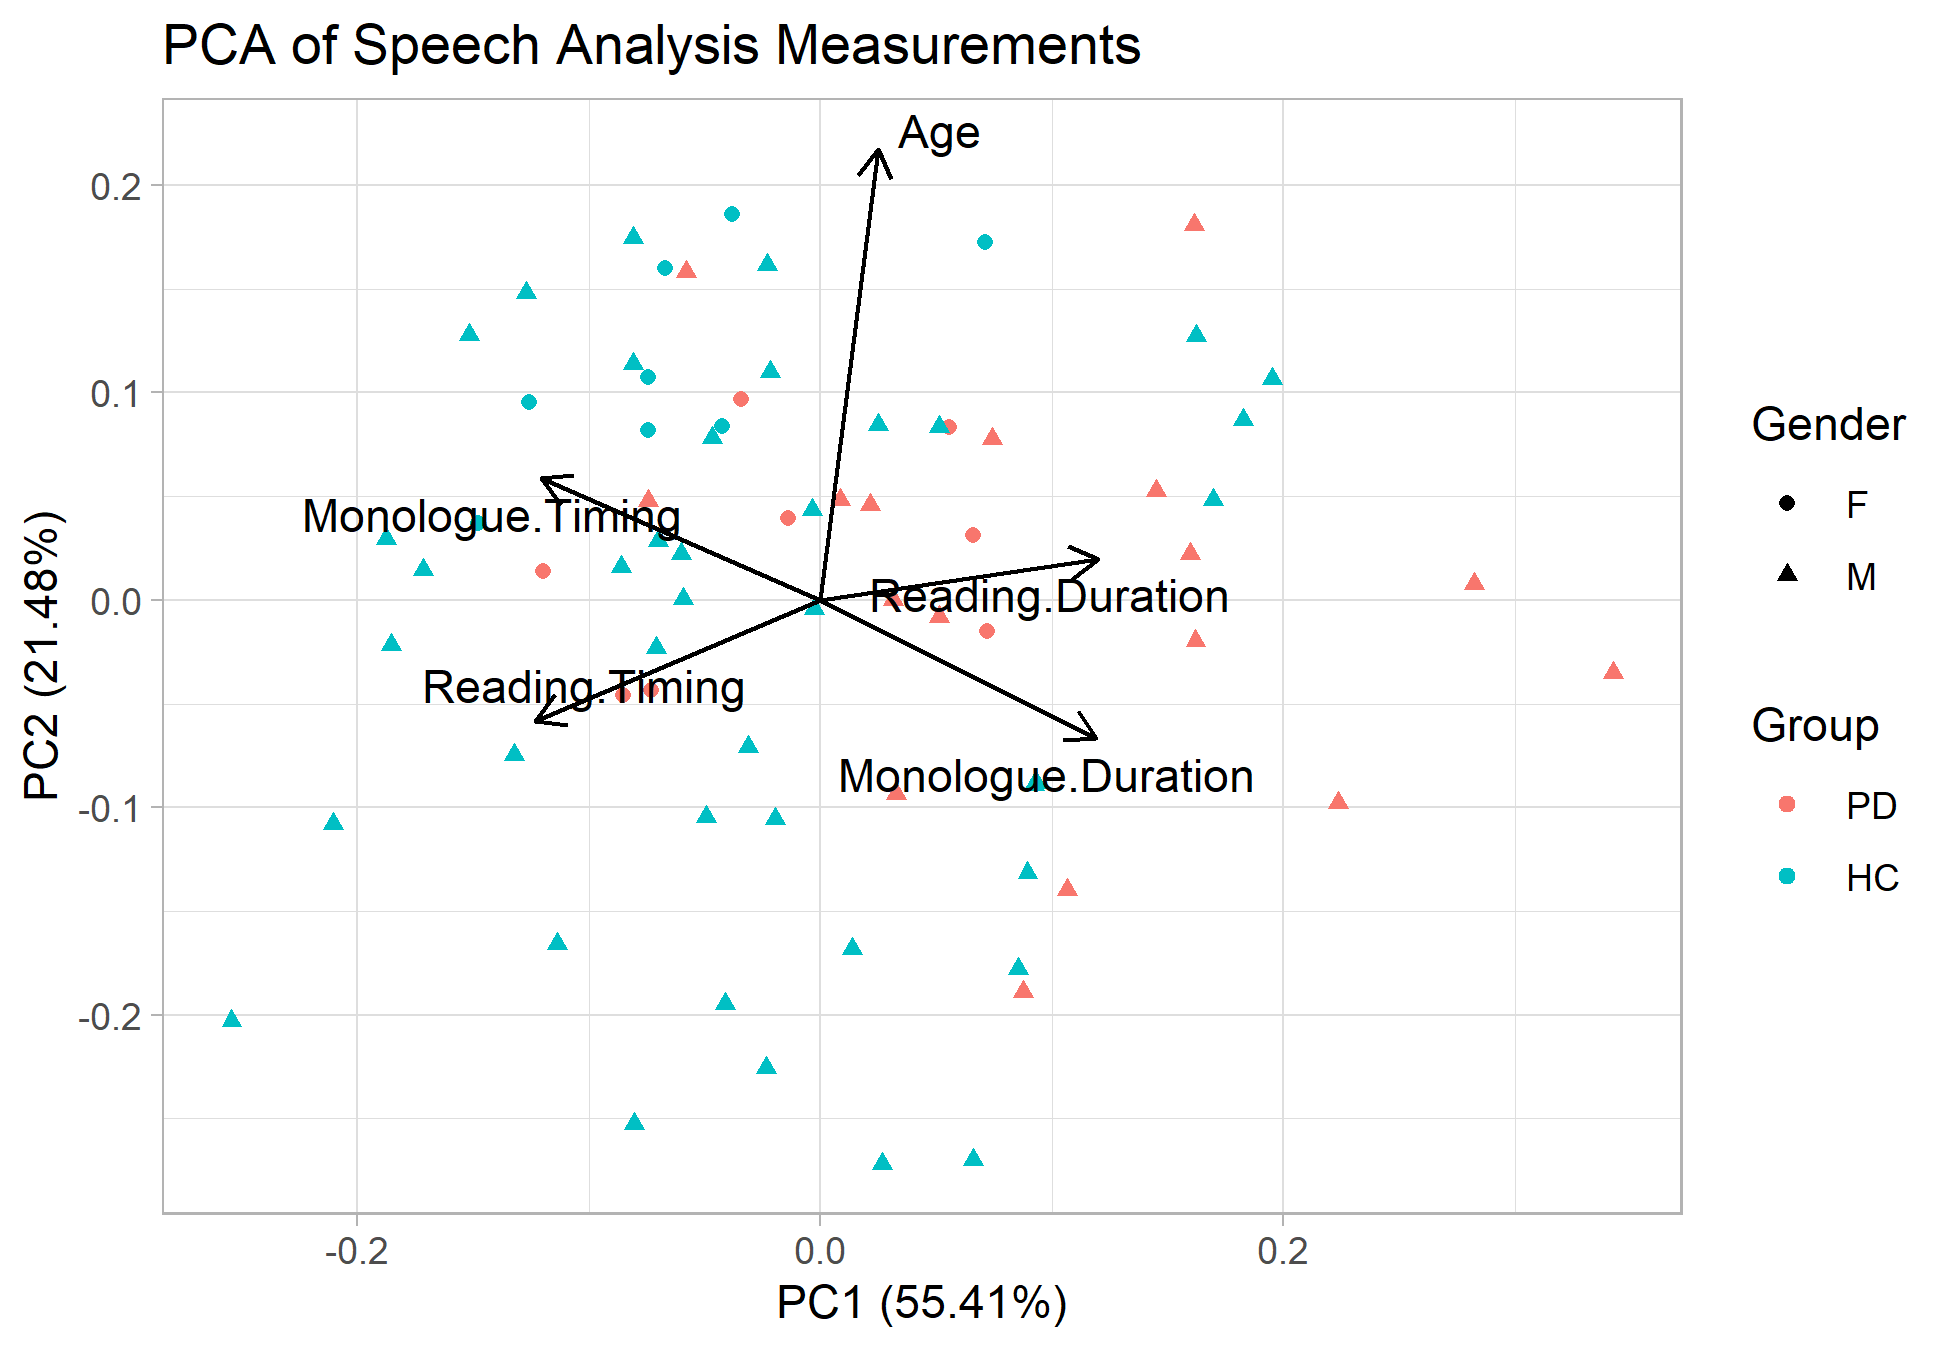
\includegraphics{dap_report_anja_probst_files/figure-latex/pca-loadings-1} 

}

\caption{How much does each variable contribute to PC1 and PC2. The varible age, contributes mainly to PC2, while the other four measured variables contribute to PC1. The arrow length represents the strength of the contribution. The gender is shown by the point shape and the group by the color.}\label{fig:pca-loadings}
\end{figure}

After creating the principal components, I reran \texttt{ggpairs}. Appendix Figure \ref{fig:pca-ggpairs} shows, that the
principal components do no longer correlate compared to the original variables (\ref{fig:correlate-ggpairs-plot}).
After experimentation with different models, the model \texttt{Group\ \textasciitilde{}\ PC1\ +\ Gender} reaches the performance
of the initial model with only two terms (Table \ref{tab:model-comparison}) and keeping the
vif low (Table \ref{tab:vif-after-pca}).

\begin{Shaded}
\begin{Highlighting}[]
\NormalTok{df.binom.pca.joined }\OtherTok{\textless{}{-}} \FunctionTok{cbind}\NormalTok{(df.binom, }\FunctionTok{predict}\NormalTok{(df.binom.pca, df.binom))}

\NormalTok{m.binom.pca }\OtherTok{\textless{}{-}} \FunctionTok{glm}\NormalTok{(}
    \AttributeTok{data =}\NormalTok{ df.binom.pca.joined[, }\SpecialCharTok{{-}}\FunctionTok{c}\NormalTok{(}\DecValTok{1}\NormalTok{, }\DecValTok{3}\NormalTok{, }\DecValTok{4}\NormalTok{, }\DecValTok{5}\NormalTok{, }\DecValTok{6}\NormalTok{)],}
\NormalTok{    Group }\SpecialCharTok{\textasciitilde{}}\NormalTok{ PC1 }\SpecialCharTok{+}\NormalTok{ Gender,}
    \AttributeTok{family =} \StringTok{"binomial"}
\NormalTok{)}
\end{Highlighting}
\end{Shaded}

\hypertarget{model-comparison-and-analysis}{%
\subsubsection{Model Comparison and Analysis}\label{model-comparison-and-analysis}}

After creating the three models (1) multiple logistic regression without interactions
\texttt{Group\ \textasciitilde{}\ Gender\ +\ Monologue.Duration\ +\ Reading.Duration} (m.binom.no.intearactions),
(2) multiple logistic regression with interactions \texttt{Group\ \textasciitilde{}\ Age\ *\ Gender\ +\ Reading.Timing\ *\ Monologue.Timing\ +\ Reading.Duration\ *\ Monologue.Duration}
(m.binom.interactions), and (3) multiple logistic regression without interactions after a PCA \texttt{Group\ \textasciitilde{}\ PC1\ +\ Gender} (m.binom.pca),
they are compared in Tables \ref{tab:model-comparison} and \ref{tab:anova}.
Model (2) with multiple interactions has the best AIC (Akaike Information Criterion) compared
to the other models, meaning that it has the lowest prediction error of the three models. In addition,
model (2) has the highest log likelihood (goodness of fit), however, given the high number of terms
compared to the other two models, this measure might be problematic. However, based on the interpretation
of the ANOVA results, model (2) is clearly better than model (1) and (3) even with a high number of
terms and the resulting lower residual degrees of freedom.

\begin{table}[!htbp] \centering 
  \caption{Comparison of logistic regression models on the data set .
    (1) Model based on automated model selection using dredge without interactions.
    (2) Model containing an interaction between Reading Duration and Monologue Duration.
    (3) Model based on principal component 1 from a PCA on the data.} 
  \label{tab:model-comparison} 
\small 
\begin{tabular}{@{\extracolsep{5pt}}lD{.}{.}{-3} D{.}{.}{-3} D{.}{.}{-3} } 
\\[-1.8ex]\hline 
\hline \\[-1.8ex] 
 & \multicolumn{3}{c}{\textit{Dependent variable:}} \\ 
\cline{2-4} 
\\[-1.8ex] & \multicolumn{3}{c}{Group} \\ 
 & \multicolumn{1}{c}{No Interactions (dredge)} & \multicolumn{1}{c}{Interactions} & \multicolumn{1}{c}{PCA} \\ 
\\[-1.8ex] & \multicolumn{1}{c}{(1)} & \multicolumn{1}{c}{(2)} & \multicolumn{1}{c}{(3)}\\ 
\hline \\[-1.8ex] 
 Constant & -0.680 & -4.231^{**} & -0.431 \\ 
  & (0.580) & (1.791) & (0.548) \\ 
  Age &  & 3.910^{**} &  \\ 
  &  & (1.995) &  \\ 
  PC1 &  &  & -0.747^{***} \\ 
  &  &  & (0.216) \\ 
  GenderM & 1.678^{**} & 4.804^{***} & 1.665^{**} \\ 
  & (0.696) & (1.832) & (0.691) \\ 
  Reading.Timing &  & 0.359 &  \\ 
  &  & (0.673) &  \\ 
  Monologue.Timing &  & 0.459 &  \\ 
  &  & (0.619) &  \\ 
  Monologue.Duration & -0.926^{**} & -1.508^{**} &  \\ 
  & (0.401) & (0.661) &  \\ 
  Age:GenderM &  & -4.820^{**} &  \\ 
  &  & (2.086) &  \\ 
  Reading.Timing:Monologue.Timing &  & 0.869^{*} &  \\ 
  &  & (0.508) &  \\ 
  Reading.Duration:Monologue.Duration &  & 0.549 &  \\ 
  &  & (0.655) &  \\ 
  Reading.Duration & -0.576 & -0.316 &  \\ 
  & (0.385) & (0.640) &  \\ 
 \hline \\[-1.8ex] 
Observations & \multicolumn{1}{c}{73} & \multicolumn{1}{c}{73} & \multicolumn{1}{c}{73} \\ 
Log Likelihood & \multicolumn{1}{c}{-37.056} & \multicolumn{1}{c}{-27.540} & \multicolumn{1}{c}{-37.536} \\ 
Akaike Inf. Crit. & \multicolumn{1}{c}{82.112} & \multicolumn{1}{c}{75.080} & \multicolumn{1}{c}{81.071} \\ 
\hline 
\hline \\[-1.8ex] 
\textit{Note:}  & \multicolumn{3}{r}{$^{*}$p$<$0.1; $^{**}$p$<$0.05; $^{***}$p$<$0.01} \\ 
\end{tabular} 
\end{table}

Inspecting the diagnostic plots for the three models (see Appendix Diagnostic Plots for Models), the residual
vs.~fitted shows a relatively hard to interpret pattern that is caused by the binomial nature of the model. It even
looks like the blue curve is close to a sigmoid curve. The normal Q-Q plots show again this binomial nature
of the data that roughly follow a normal distribution, however, the data points are split in two parts, where
one of the parts seems to follow a normal distribution while the other does not.
The scale-location plots show a similar pattern for all
models. the line is far from horizontal, which would mean that the assumption of homoscedasticity is not
satisfied. However, there is again a clear pattern that could be caused by diagnosing a logistic rather than
a linear regression. The plots showing Cook's distance only show one outlier with a distance of more than 0.5
in the model with many interactions.

However, even if model (2) should be chosen according to it's AIC and ANOVA results, the high number of
terms combined with the collinearity based on the VIF analysis, made model (3) \texttt{Group\ \textasciitilde{}\ PC1\ +\ Gender} my
model of choice. I proceeded to evaluate the model based on a training testing split using the function
shown in Appendix Functions. The results show an overall accuracy of 68.4\% with a sensitivity for detecting
Parkinson's of 57.10\% and a specificity of
75\%.

\begin{table}[!htbp] \centering 
  \caption{Comparison of models using ANOVA} 
  \label{tab:anova} 
\begin{tabular}{@{\extracolsep{5pt}} cccccc} 
\\[-1.8ex]\hline 
\hline \\[-1.8ex] 
 & Resid. Df & Resid. Dev & Df & Deviance & Pr(\textgreater Chi) \\ 
\hline \\[-1.8ex] 
1 & $69$ & $74.112$ & $$ & $$ & $$ \\ 
2 & $63$ & $55.080$ & $6$ & $19.032$ & $0.004$ \\ 
3 & $70$ & $75.071$ & $$-$7$ & $$-$19.991$ & $0.006$ \\ 
\hline \\[-1.8ex] 
\end{tabular} 
\end{table}

\clearpage

\hypertarget{multinomial-regression}{%
\subsection{Multinomial Regression}\label{multinomial-regression}}

To predict over all three groups (HC, PD, RBD), I have to use a more complex
multinomial model. However, as the 3 groups are unbalanced, I chose to subsample
the groups HC (\(n=48\) after outlier removal) and RBD (\(n=48\) after outlier removal) to
match the size of the group PD (\(n = 25\) after outlier removal). While I did not do this for
the binomial logistic regression, I chose to do it here to make the task hopefully easier.
In order to evaluate the multinomial model, I created a train and test set.
The training set contains 75\% of the observations, while the test set contains the
remaining 25\%. The split was done considering the groups to avoid over- or underrepresentation
of one group in either the training or the testing set.
The functions for training and testing as well as plotting are shown in the
Appendix Functions.

\begin{figure}

{\centering 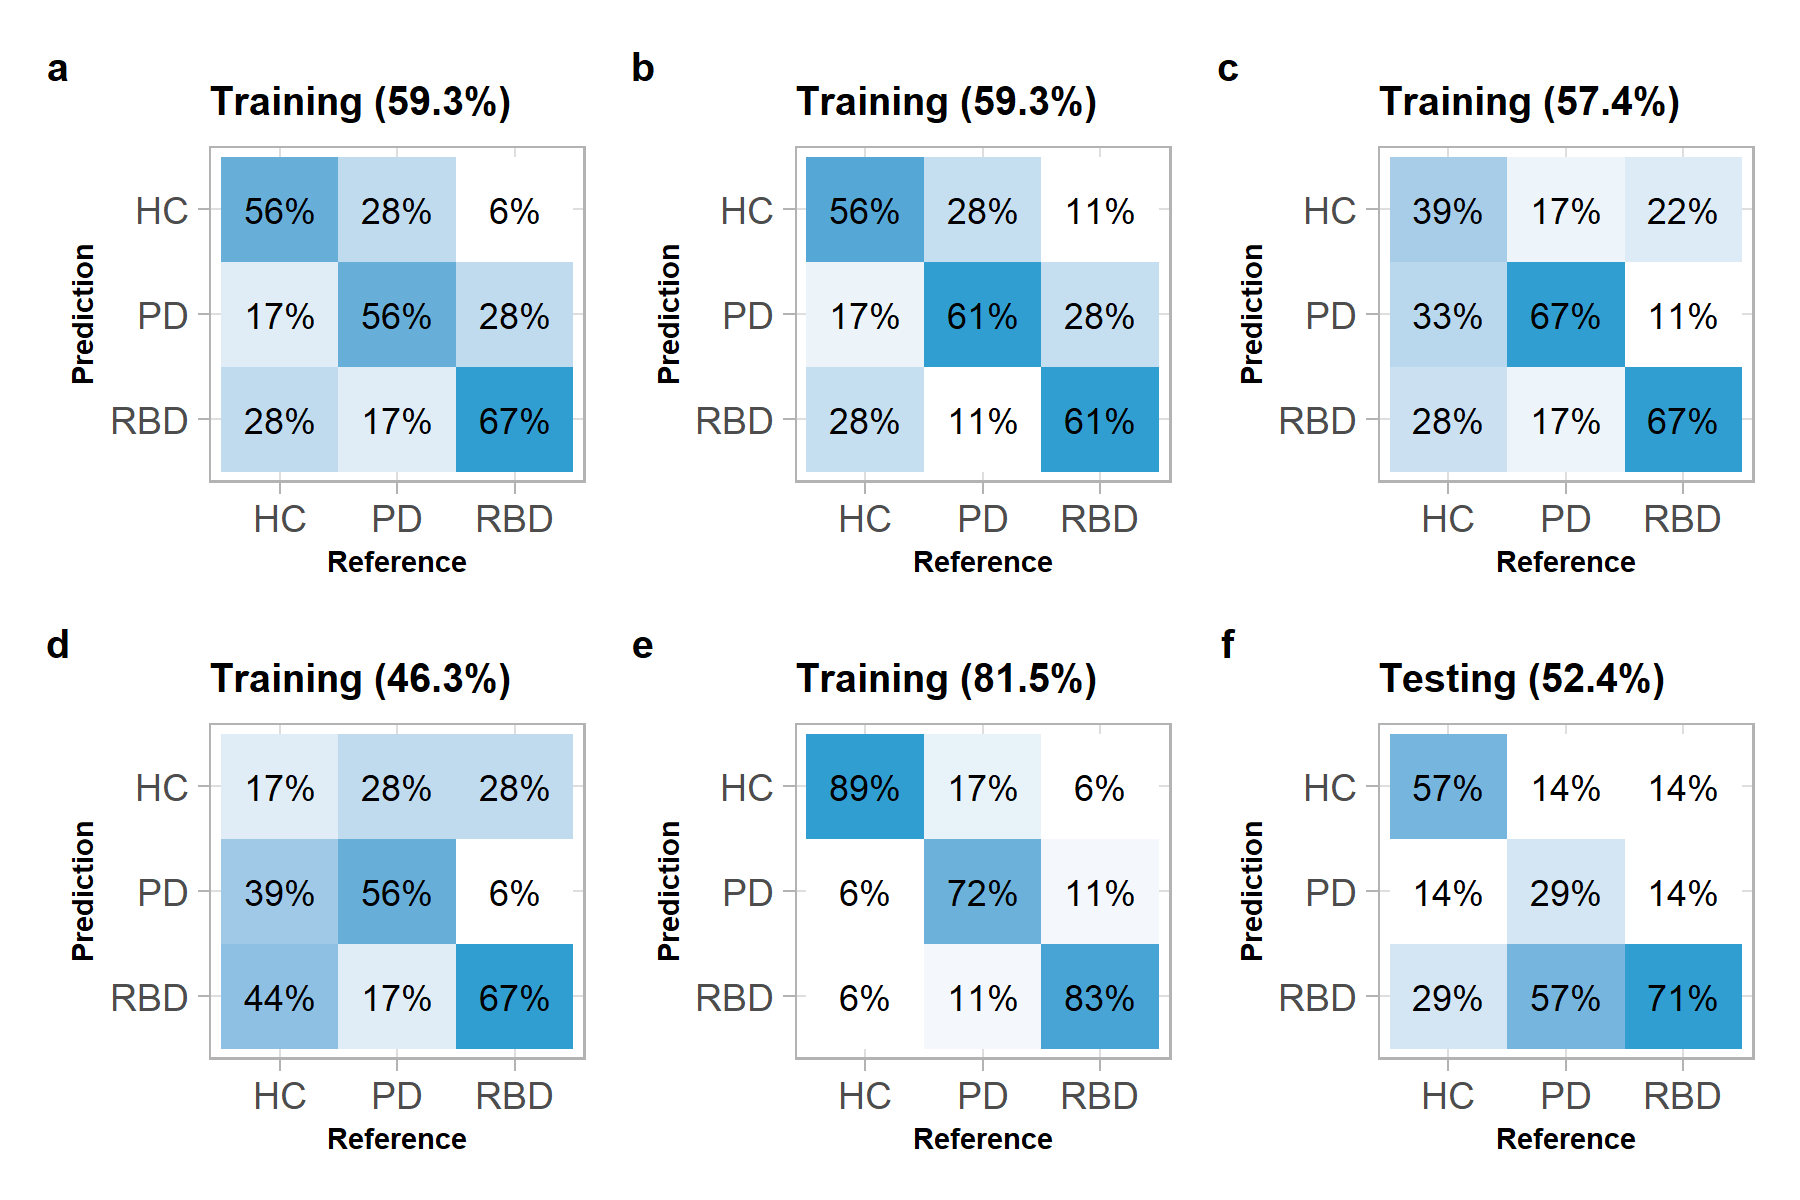
\includegraphics{dap_report_anja_probst_files/figure-latex/multinomial-regression-1} 

}

\caption{Confusion matrices of the training set evaluation (a-e, corresponding to models a-e) and the final test set evaluation based on model (c).}\label{fig:multinomial-regression}
\end{figure}

The performance and confusion matrices of the models considered during the model selection process are shown in Figure
\ref{fig:multinomial-regression} and the ANOVA output in Table \ref{tab:multinom-anova} (models in same order of the figure).
The initial full model (a) \texttt{Group\ \textasciitilde{}\ .} (\(AIC = 121.254\)) reaches a training accuracy of 59.3\%.
Removing the variable Age from the model (b) \texttt{Group\ \textasciitilde{}\ .\ -\ Age}, decreases the AIC to \(120.6\) while keeping the training accuracy at 59.3\%.
Removing any further variables does not lead to a decrease in AIC or an increase in training accuracy, this is examplified
by the model (c) \texttt{Group\ \textasciitilde{}\ .\ -\ Age\ -\ Reading.Timing}, where the variable Reading Timing was removed based on effect size
and the AIC increased to \(121.538\) and the training accuracy
dropped to 57.4\%. Until now, none of the ANOVA results show a significant change. Removing the variable Monologue Timing in model (d) \texttt{Group\ \textasciitilde{}\ .\ -\ Age\ -\ Reading.Timing\ -\ Monologue.Timing}
reduced the AIC to 119.305 and doesn't effect the model significantly. However, the training accuracy drops by more than 10\%
to 46.3\%. For this reason, I chose to stop removing variables from the model and end the model selection process.
As an experiment I added a significant amount of interactions in model (e) \texttt{Group\ \textasciitilde{}\ Monologue.Duration\ *\ Reading.Duration\ *\ Monologue.Timing\ *\ Reading.Timing},
which increases the AIC to 123.742. This model is significantly better according to ANOVA and has an excellent
training accuracy of 81.5\%. However, given the number of terms in this model, I assume this to be a case of overfitting, as this
doesn't seem like a realistic result compared to my experience with this data. Based on the training accuracy and the AIC as well
as the ANOVA, I chose model (c) as the model to run the test on. The resulting confusion matrix of the test based on the model
\texttt{Group\ \textasciitilde{}\ .\ -\ Age\ -\ Reading.Timing} can be seen in Figure \ref{fig:multinomial-regression} f.~The model shows an overall accuracy of 52.4\%.
It seems to be especially good at identifying cases of REM sleep behaviour disorder, with 71\% of correct predictions. On the other hand,
the model misclassifies 57\% of Parkinson's disease cases as RDB, which would of course be a substantial problem in a clinical setting.
Specifically, the model detects Parkinson's with a sensitivity of 50\% and a specificity of
70.60\%.

\begin{table}[!htbp] \centering 
  \caption{Comparison of multinomial models using ANOVA} 
  \label{tab:multinom-anova} 
\begin{tabular}{@{\extracolsep{5pt}} cccccccc} 
\\[-1.8ex]\hline 
\hline \\[-1.8ex] 
 & Resid. df & Resid. Dev & Test &    Df & LR stat. & Pr(Chi) \\ 
\hline \\[-1.8ex] 
1 & $100$ & $103.305$ &  & $$ & $$ & $$ \\ 
2 & $98$ & $101.538$ & 1 vs 2 & $2$ & $1.767$ & $0.413$ \\ 
3 & $96$ & $96.601$ & 2 vs 3 & $2$ & $4.938$ & $0.085$ \\ 
4 & $94$ & $93.254$ & 3 vs 4 & $2$ & $3.347$ & $0.188$ \\ 
5 & $76$ & $59.742$ & 4 vs 5 & $18$ & $33.512$ & $0.014$ \\ 
\hline \\[-1.8ex] 
\end{tabular} 
\end{table}

\clearpage

\hypertarget{conclusion}{%
\section{Conclusion}\label{conclusion}}

Given the challenging nature of the data set, as well as the collinearity within it, the multinomial model
yielded surprisingly good performance when diagnosing REM sleep behaviour disorder subjects but a very low
performance when diagnosing subjects with Parkinson's disease. A major issue in addition to the nature of
the data (the strong correlations among most of the predictors) was the low amount of data, especially the
Parkinson's disease group (\(n=25\) after outlier removal). This in turn lead to even smaller training and
testing sets. However, as the authors of the original study have shown, the data is sufficient to conclude
that they have found significant features that can be used to detect early patterns of neurodegeneration.
To come back to my initial hypothesis, that there are speech related cues, which could help to detect
Parkinson\texttt{s\ disease\ in\ an\ earlier\ stage\ and\ also\ help\ to\ distinguish\ between\ Parkinson}s disease and
REM sleep behaviour disorder, the results show, that based on the available data, I was not able to
create a robust predictive model with high accuracy.

In addition, I have shown that reducing the problem to a binomial problem by only trying to distinguish
between healthy controls and subjects with Parkinson's disease can be achieved with a sensitivity of 75\%
and a specificity of 57.1\% using a binomial logistic regression model.

Overall, the outcome of this project has been educatually valuable. However, the models that resulted from
it are probably too simple to achive high enough accuracies to be of value.

\clearpage

\hypertarget{appendix}{%
\section{Appendix}\label{appendix}}

\hypertarget{functions}{%
\subsection{Functions}\label{functions}}

The following function was used to assess binomial models

\begin{Shaded}
\begin{Highlighting}[]
\NormalTok{evaluate.binom.model }\OtherTok{\textless{}{-}} \ControlFlowTok{function}\NormalTok{(formula, data) \{}
    \FunctionTok{set.seed}\NormalTok{(}\DecValTok{123}\NormalTok{)}

\NormalTok{    data.split }\OtherTok{\textless{}{-}} \FunctionTok{initial\_split}\NormalTok{(data, }\AttributeTok{prop =} \FloatTok{0.75}\NormalTok{, }\AttributeTok{strata =}\NormalTok{ Group)}
\NormalTok{    df.train }\OtherTok{\textless{}{-}} \FunctionTok{training}\NormalTok{(data.split)}
\NormalTok{    df.test }\OtherTok{\textless{}{-}} \FunctionTok{testing}\NormalTok{(data.split)}

\NormalTok{    m }\OtherTok{\textless{}{-}} \FunctionTok{glm}\NormalTok{(formula, }\AttributeTok{data =}\NormalTok{ df.train, }\AttributeTok{family =}\NormalTok{ binomial)}

\NormalTok{    df.test}\SpecialCharTok{$}\NormalTok{Group.Predicted }\OtherTok{\textless{}{-}} \FunctionTok{relevel}\NormalTok{(}
        \FunctionTok{as.factor}\NormalTok{(}\FunctionTok{ifelse}\NormalTok{(}
            \FunctionTok{predict}\NormalTok{(m, }\AttributeTok{newdata =}\NormalTok{ df.test, }\StringTok{"response"}\NormalTok{) }\SpecialCharTok{\textgreater{}=} \FloatTok{0.5}\NormalTok{, }
            \StringTok{"HC"}\NormalTok{, }\StringTok{"PD"}
\NormalTok{        )), }\AttributeTok{ref=}\StringTok{"PD"}
\NormalTok{    )}
\NormalTok{    cm }\OtherTok{\textless{}{-}} \FunctionTok{confusionMatrix}\NormalTok{(df.test}\SpecialCharTok{$}\NormalTok{Group, df.test}\SpecialCharTok{$}\NormalTok{Group.Predicted)}

    \FunctionTok{return}\NormalTok{(}\FunctionTok{list}\NormalTok{(}\AttributeTok{cm =}\NormalTok{ cm, }\AttributeTok{model =}\NormalTok{ m))}
\NormalTok{\}}

\NormalTok{l }\OtherTok{=} \FunctionTok{evaluate.binom.model}\NormalTok{(}
\NormalTok{    Group }\SpecialCharTok{\textasciitilde{}}\NormalTok{ PC1 }\SpecialCharTok{+}\NormalTok{ Gender, }
\NormalTok{    df.binom.pca.joined[, }\SpecialCharTok{{-}}\FunctionTok{c}\NormalTok{(}\DecValTok{1}\NormalTok{, }\DecValTok{3}\NormalTok{, }\DecValTok{4}\NormalTok{, }\DecValTok{5}\NormalTok{, }\DecValTok{6}\NormalTok{)]}
\NormalTok{)}
\end{Highlighting}
\end{Shaded}

The following two are functions were used to evaluate and visualize the multinomial models.

\begin{Shaded}
\begin{Highlighting}[]
\NormalTok{evaluate.multinom.model }\OtherTok{\textless{}{-}} \ControlFlowTok{function}\NormalTok{(formula, data, test) \{}
    \FunctionTok{set.seed}\NormalTok{(}\DecValTok{123}\NormalTok{)}

\NormalTok{    data.split }\OtherTok{\textless{}{-}} \FunctionTok{initial\_split}\NormalTok{(data, }\AttributeTok{prop =} \FloatTok{0.75}\NormalTok{, }\AttributeTok{strata =}\NormalTok{ Group)}
\NormalTok{    df.train }\OtherTok{\textless{}{-}} \FunctionTok{training}\NormalTok{(data.split)}
\NormalTok{    df.test }\OtherTok{\textless{}{-}} \FunctionTok{testing}\NormalTok{(data.split)}

\NormalTok{    m }\OtherTok{\textless{}{-}} \FunctionTok{multinom}\NormalTok{(formula, }\AttributeTok{data =}\NormalTok{ df.train, }\AttributeTok{maxit =} \DecValTok{200}\NormalTok{)}

    \ControlFlowTok{if}\NormalTok{ (test }\SpecialCharTok{==} \ConstantTok{TRUE}\NormalTok{) \{}
\NormalTok{        df.test}\SpecialCharTok{$}\NormalTok{Group.Predicted }\OtherTok{\textless{}{-}} \FunctionTok{predict}\NormalTok{(m, }\AttributeTok{newdata =}\NormalTok{ df.test, }\StringTok{"class"}\NormalTok{)}
\NormalTok{        cm }\OtherTok{\textless{}{-}} \FunctionTok{confusionMatrix}\NormalTok{(df.test}\SpecialCharTok{$}\NormalTok{Group, df.test}\SpecialCharTok{$}\NormalTok{Group.Predicted)}

        \FunctionTok{return}\NormalTok{(}\FunctionTok{list}\NormalTok{(}\AttributeTok{cm =}\NormalTok{ cm, }\AttributeTok{model =}\NormalTok{ m))}
\NormalTok{    \} }\ControlFlowTok{else}\NormalTok{ \{}
\NormalTok{        df.train}\SpecialCharTok{$}\NormalTok{Group.Predicted }\OtherTok{\textless{}{-}} \FunctionTok{predict}\NormalTok{(m, }\AttributeTok{newdata =}\NormalTok{ df.train, }\StringTok{"class"}\NormalTok{)}
\NormalTok{        cm }\OtherTok{\textless{}{-}} \FunctionTok{confusionMatrix}\NormalTok{(df.train}\SpecialCharTok{$}\NormalTok{Group, df.train}\SpecialCharTok{$}\NormalTok{Group.Predicted)}

        \FunctionTok{return}\NormalTok{(}\FunctionTok{list}\NormalTok{(}\AttributeTok{cm =}\NormalTok{ cm, }\AttributeTok{model =}\NormalTok{ m))}
\NormalTok{    \}}
\NormalTok{\}}
\end{Highlighting}
\end{Shaded}

\begin{Shaded}
\begin{Highlighting}[]
\NormalTok{plot\_cm }\OtherTok{\textless{}{-}} \ControlFlowTok{function}\NormalTok{(cm, tag, title) \{}
    \CommentTok{\# Adapted from https://stackoverflow.com/questions}
    \CommentTok{\# /37897252/plot{-}confusion{-}matrix{-}in{-}r{-}using{-}ggplot}

\NormalTok{    cm.df }\OtherTok{\textless{}{-}} \FunctionTok{data.frame}\NormalTok{(}\FunctionTok{prop.table}\NormalTok{(cm}\SpecialCharTok{$}\NormalTok{table, }\AttributeTok{margin =} \DecValTok{1}\NormalTok{))}
\NormalTok{    cm.df}\SpecialCharTok{$}\NormalTok{Prediction }\OtherTok{\textless{}{-}} \FunctionTok{factor}\NormalTok{(}
\NormalTok{        cm.df}\SpecialCharTok{$}\NormalTok{Prediction,}
        \AttributeTok{levels =} \FunctionTok{rev}\NormalTok{(}\FunctionTok{levels}\NormalTok{(cm.df}\SpecialCharTok{$}\NormalTok{Prediction))}
\NormalTok{    )}

\NormalTok{    accuracy }\OtherTok{\textless{}{-}} \FunctionTok{round}\NormalTok{(cm}\SpecialCharTok{$}\NormalTok{overall[[}\StringTok{"Accuracy"}\NormalTok{]], }\DecValTok{3}\NormalTok{) }\SpecialCharTok{*} \DecValTok{100}

\NormalTok{    p }\OtherTok{\textless{}{-}} \FunctionTok{ggplot}\NormalTok{(cm.df, }\FunctionTok{aes}\NormalTok{(Prediction, Reference, }\AttributeTok{fill =}\NormalTok{ Freq)) }\SpecialCharTok{+}
        \FunctionTok{geom\_tile}\NormalTok{(}\AttributeTok{show.legend =} \ConstantTok{FALSE}\NormalTok{) }\SpecialCharTok{+}
        \FunctionTok{geom\_text}\NormalTok{(}
            \FunctionTok{aes}\NormalTok{(}\AttributeTok{label =}\NormalTok{ scales}\SpecialCharTok{::}\FunctionTok{percent}\NormalTok{(Freq, }\AttributeTok{accuracy =} \DecValTok{1}\NormalTok{)),}
            \AttributeTok{size =} \DecValTok{3}
\NormalTok{        ) }\SpecialCharTok{+}
        \FunctionTok{scale\_fill\_gradient}\NormalTok{(}\AttributeTok{low =} \StringTok{"white"}\NormalTok{, }\AttributeTok{high =} \StringTok{"\#319ed1"}\NormalTok{) }\SpecialCharTok{+}
        \FunctionTok{labs}\NormalTok{(}
            \AttributeTok{title =} \FunctionTok{paste}\NormalTok{(title, }\StringTok{" ("}\NormalTok{, accuracy, }\StringTok{"\%)"}\NormalTok{, }\AttributeTok{sep =} \StringTok{""}\NormalTok{),}
            \AttributeTok{x =} \StringTok{"Reference"}\NormalTok{, }\AttributeTok{y =} \StringTok{"Prediction"}\NormalTok{, }\AttributeTok{tag =}\NormalTok{ tag}
\NormalTok{        ) }\SpecialCharTok{+}
        \FunctionTok{scale\_x\_discrete}\NormalTok{(}\AttributeTok{labels =} \FunctionTok{c}\NormalTok{(}\StringTok{"HC"}\NormalTok{, }\StringTok{"PD"}\NormalTok{, }\StringTok{"RBD"}\NormalTok{)) }\SpecialCharTok{+}
        \FunctionTok{scale\_y\_discrete}\NormalTok{(}\AttributeTok{labels =} \FunctionTok{c}\NormalTok{(}\StringTok{"RBD"}\NormalTok{, }\StringTok{"PD"}\NormalTok{, }\StringTok{"HC"}\NormalTok{)) }\SpecialCharTok{+}
        \FunctionTok{theme\_light}\NormalTok{() }\SpecialCharTok{+}
        \FunctionTok{theme}\NormalTok{(}
            \AttributeTok{plot.tag =} \FunctionTok{element\_text}\NormalTok{(),}
            \AttributeTok{title =} \FunctionTok{element\_text}\NormalTok{(}\AttributeTok{size =} \DecValTok{8}\NormalTok{, }\AttributeTok{face =} \StringTok{"bold"}\NormalTok{),}
            \AttributeTok{axis.title =} \FunctionTok{element\_text}\NormalTok{(}\AttributeTok{size =} \DecValTok{7}\NormalTok{, }\AttributeTok{face =} \StringTok{"bold"}\NormalTok{)}
\NormalTok{        )}

    \FunctionTok{return}\NormalTok{(p)}
\NormalTok{\}}
\end{Highlighting}
\end{Shaded}

\hypertarget{logistic-regression-with-intereactions}{%
\subsection{Logistic Regression with Intereactions}\label{logistic-regression-with-intereactions}}

\begin{verbatim}
Warning: glm.fit: fitted probabilities numerically 0 or 1 occurred
\end{verbatim}

\begin{verbatim}
Call:
glm(formula = Group ~ Age * Gender + Monologue.Duration * Monologue.Timing * 
    Reading.Duration * Reading.Timing, family = binomial, data = df.binom)

Deviance Residuals: 
     Min        1Q    Median        3Q       Max  
-1.98317  -0.33996   0.07333   0.47703   1.80759  

Coefficients:
                                                                    Estimate
(Intercept)                                                          -5.4879
Age                                                                   4.5684
GenderM                                                               6.3624
Monologue.Duration                                                   -2.1706
Monologue.Timing                                                     -0.1611
Reading.Duration                                                     -0.5101
Reading.Timing                                                        0.7153
Age:GenderM                                                          -5.5255
Monologue.Duration:Monologue.Timing                                   0.3333
Monologue.Duration:Reading.Duration                                   0.9567
Monologue.Timing:Reading.Duration                                    -1.2211
Monologue.Duration:Reading.Timing                                     0.1528
Monologue.Timing:Reading.Timing                                       2.7304
Reading.Duration:Reading.Timing                                       0.3704
Monologue.Duration:Monologue.Timing:Reading.Duration                  0.3122
Monologue.Duration:Monologue.Timing:Reading.Timing                   -0.3689
Monologue.Duration:Reading.Duration:Reading.Timing                   -1.9001
Monologue.Timing:Reading.Duration:Reading.Timing                     -2.2662
Monologue.Duration:Monologue.Timing:Reading.Duration:Reading.Timing  -0.2252
                                                                    Std. Error
(Intercept)                                                             2.5760
Age                                                                     2.6273
GenderM                                                                 2.6104
Monologue.Duration                                                      1.0413
Monologue.Timing                                                        0.8972
Reading.Duration                                                        0.8666
Reading.Timing                                                          0.8935
Age:GenderM                                                             2.7366
Monologue.Duration:Monologue.Timing                                     0.8314
Monologue.Duration:Reading.Duration                                     1.4365
Monologue.Timing:Reading.Duration                                       1.4922
Monologue.Duration:Reading.Timing                                       1.6574
Monologue.Timing:Reading.Timing                                         1.3546
Reading.Duration:Reading.Timing                                         0.7779
Monologue.Duration:Monologue.Timing:Reading.Duration                    1.0315
Monologue.Duration:Monologue.Timing:Reading.Timing                      1.5813
Monologue.Duration:Reading.Duration:Reading.Timing                      1.8127
Monologue.Timing:Reading.Duration:Reading.Timing                        1.4973
Monologue.Duration:Monologue.Timing:Reading.Duration:Reading.Timing     1.5820
                                                                    z value
(Intercept)                                                          -2.130
Age                                                                   1.739
GenderM                                                               2.437
Monologue.Duration                                                   -2.085
Monologue.Timing                                                     -0.180
Reading.Duration                                                     -0.589
Reading.Timing                                                        0.801
Age:GenderM                                                          -2.019
Monologue.Duration:Monologue.Timing                                   0.401
Monologue.Duration:Reading.Duration                                   0.666
Monologue.Timing:Reading.Duration                                    -0.818
Monologue.Duration:Reading.Timing                                     0.092
Monologue.Timing:Reading.Timing                                       2.016
Reading.Duration:Reading.Timing                                       0.476
Monologue.Duration:Monologue.Timing:Reading.Duration                  0.303
Monologue.Duration:Monologue.Timing:Reading.Timing                   -0.233
Monologue.Duration:Reading.Duration:Reading.Timing                   -1.048
Monologue.Timing:Reading.Duration:Reading.Timing                     -1.513
Monologue.Duration:Monologue.Timing:Reading.Duration:Reading.Timing  -0.142
                                                                    Pr(>|z|)  
(Intercept)                                                           0.0331 *
Age                                                                   0.0821 .
GenderM                                                               0.0148 *
Monologue.Duration                                                    0.0371 *
Monologue.Timing                                                      0.8575  
Reading.Duration                                                      0.5561  
Reading.Timing                                                        0.4234  
Age:GenderM                                                           0.0435 *
Monologue.Duration:Monologue.Timing                                   0.6885  
Monologue.Duration:Reading.Duration                                   0.5054  
Monologue.Timing:Reading.Duration                                     0.4132  
Monologue.Duration:Reading.Timing                                     0.9265  
Monologue.Timing:Reading.Timing                                       0.0438 *
Reading.Duration:Reading.Timing                                       0.6340  
Monologue.Duration:Monologue.Timing:Reading.Duration                  0.7621  
Monologue.Duration:Monologue.Timing:Reading.Timing                    0.8155  
Monologue.Duration:Reading.Duration:Reading.Timing                    0.2945  
Monologue.Timing:Reading.Duration:Reading.Timing                      0.1302  
Monologue.Duration:Monologue.Timing:Reading.Duration:Reading.Timing   0.8868  
---
Signif. codes:  0 '***' 0.001 '**' 0.01 '*' 0.05 '.' 0.1 ' ' 1

(Dispersion parameter for binomial family taken to be 1)

    Null deviance: 93.828  on 72  degrees of freedom
Residual deviance: 46.997  on 54  degrees of freedom
AIC: 84.997

Number of Fisher Scoring iterations: 9
\end{verbatim}

\begin{verbatim}
Warning: glm.fit: fitted probabilities numerically 0 or 1 occurred
\end{verbatim}

\begin{verbatim}
Call:
glm(formula = Group ~ Age * Gender * Monologue.Duration * Monologue.Timing + 
    Reading.Duration * Reading.Timing, family = binomial, data = df.binom)

Deviance Residuals: 
     Min        1Q    Median        3Q       Max  
-1.96791  -0.00015   0.13882   0.54220   1.75620  

Coefficients:
                                                  Estimate Std. Error z value
(Intercept)                                     -5.021e+01  1.874e+04  -0.003
Age                                             -1.357e+01  2.353e+04  -0.001
GenderM                                          5.071e+01  1.874e+04   0.003
Monologue.Duration                              -3.320e+01  6.600e+04  -0.001
Monologue.Timing                                 1.342e+02  1.532e+04   0.009
Reading.Duration                                -7.937e-01  8.570e-01  -0.926
Reading.Timing                                  -3.765e-01  8.594e-01  -0.438
Age:GenderM                                      1.278e+01  2.353e+04   0.001
Age:Monologue.Duration                          -2.719e+01  1.024e+05   0.000
GenderM:Monologue.Duration                       3.244e+01  6.600e+04   0.000
Age:Monologue.Timing                            -1.190e+02  1.995e+04  -0.006
GenderM:Monologue.Timing                        -1.336e+02  1.532e+04  -0.009
Monologue.Duration:Monologue.Timing              1.104e+02  7.512e+04   0.001
Reading.Duration:Reading.Timing                 -5.665e-01  5.833e-01  -0.971
Age:GenderM:Monologue.Duration                   2.731e+01  1.024e+05   0.000
Age:GenderM:Monologue.Timing                     1.196e+02  1.995e+04   0.006
Age:Monologue.Duration:Monologue.Timing         -1.527e+02  7.818e+04  -0.002
GenderM:Monologue.Duration:Monologue.Timing     -1.105e+02  7.512e+04  -0.001
Age:GenderM:Monologue.Duration:Monologue.Timing  1.534e+02  7.818e+04   0.002
                                                Pr(>|z|)
(Intercept)                                        0.998
Age                                                1.000
GenderM                                            0.998
Monologue.Duration                                 1.000
Monologue.Timing                                   0.993
Reading.Duration                                   0.354
Reading.Timing                                     0.661
Age:GenderM                                        1.000
Age:Monologue.Duration                             1.000
GenderM:Monologue.Duration                         1.000
Age:Monologue.Timing                               0.995
GenderM:Monologue.Timing                           0.993
Monologue.Duration:Monologue.Timing                0.999
Reading.Duration:Reading.Timing                    0.331
Age:GenderM:Monologue.Duration                     1.000
Age:GenderM:Monologue.Timing                       0.995
Age:Monologue.Duration:Monologue.Timing            0.998
GenderM:Monologue.Duration:Monologue.Timing        0.999
Age:GenderM:Monologue.Duration:Monologue.Timing    0.998

(Dispersion parameter for binomial family taken to be 1)

    Null deviance: 93.828  on 72  degrees of freedom
Residual deviance: 48.623  on 54  degrees of freedom
AIC: 86.623

Number of Fisher Scoring iterations: 19
\end{verbatim}

\begin{verbatim}
Call:
glm(formula = Group ~ Age * Gender + Monologue.Duration * Monologue.Timing + 
    Reading.Duration * Reading.Timing, family = binomial, data = df.binom)

Deviance Residuals: 
    Min       1Q   Median       3Q      Max  
-2.0950  -0.4979   0.2877   0.6317   1.6246  

Coefficients:
                                      Estimate Std. Error z value Pr(>|z|)   
(Intercept)                         -3.5767824  1.5612509  -2.291  0.02197 * 
Age                                  3.6063514  1.7491085   2.062  0.03922 * 
GenderM                              4.0792578  1.5553206   2.623  0.00872 **
Monologue.Duration                  -1.1957236  0.6322390  -1.891  0.05859 . 
Monologue.Timing                     0.2690058  0.5733037   0.469  0.63891   
Reading.Duration                    -0.6926199  0.6389234  -1.084  0.27835   
Reading.Timing                      -0.0007886  0.6081766  -0.001  0.99897   
Age:GenderM                         -4.4071881  1.8356945  -2.401  0.01636 * 
Monologue.Duration:Monologue.Timing -0.2244089  0.3720875  -0.603  0.54644   
Reading.Duration:Reading.Timing     -0.5708029  0.4774547  -1.196  0.23189   
---
Signif. codes:  0 '***' 0.001 '**' 0.01 '*' 0.05 '.' 0.1 ' ' 1

(Dispersion parameter for binomial family taken to be 1)

    Null deviance: 93.828  on 72  degrees of freedom
Residual deviance: 59.566  on 63  degrees of freedom
AIC: 79.566

Number of Fisher Scoring iterations: 6
\end{verbatim}

\begin{verbatim}
Call:
glm(formula = Group ~ Age * Gender + Reading.Timing * Monologue.Timing + 
    Reading.Duration * Monologue.Duration, family = binomial, 
    data = df.binom)

Deviance Residuals: 
    Min       1Q   Median       3Q      Max  
-2.0509  -0.4299   0.2311   0.6270   1.9248  

Coefficients:
                                    Estimate Std. Error z value Pr(>|z|)   
(Intercept)                          -4.2306     1.7907  -2.363  0.01815 * 
Age                                   3.9099     1.9945   1.960  0.04996 * 
GenderM                               4.8035     1.8322   2.622  0.00875 **
Reading.Timing                        0.3587     0.6726   0.533  0.59380   
Monologue.Timing                      0.4592     0.6190   0.742  0.45815   
Reading.Duration                     -0.3157     0.6403  -0.493  0.62195   
Monologue.Duration                   -1.5081     0.6605  -2.283  0.02243 * 
Age:GenderM                          -4.8196     2.0855  -2.311  0.02083 * 
Reading.Timing:Monologue.Timing       0.8691     0.5079   1.711  0.08703 . 
Reading.Duration:Monologue.Duration   0.5485     0.6548   0.838  0.40224   
---
Signif. codes:  0 '***' 0.001 '**' 0.01 '*' 0.05 '.' 0.1 ' ' 1

(Dispersion parameter for binomial family taken to be 1)

    Null deviance: 93.828  on 72  degrees of freedom
Residual deviance: 55.080  on 63  degrees of freedom
AIC: 75.08

Number of Fisher Scoring iterations: 6
\end{verbatim}

\hypertarget{pca-appendix}{%
\subsection{PCA Appendix}\label{pca-appendix}}

\begin{figure}
\centering
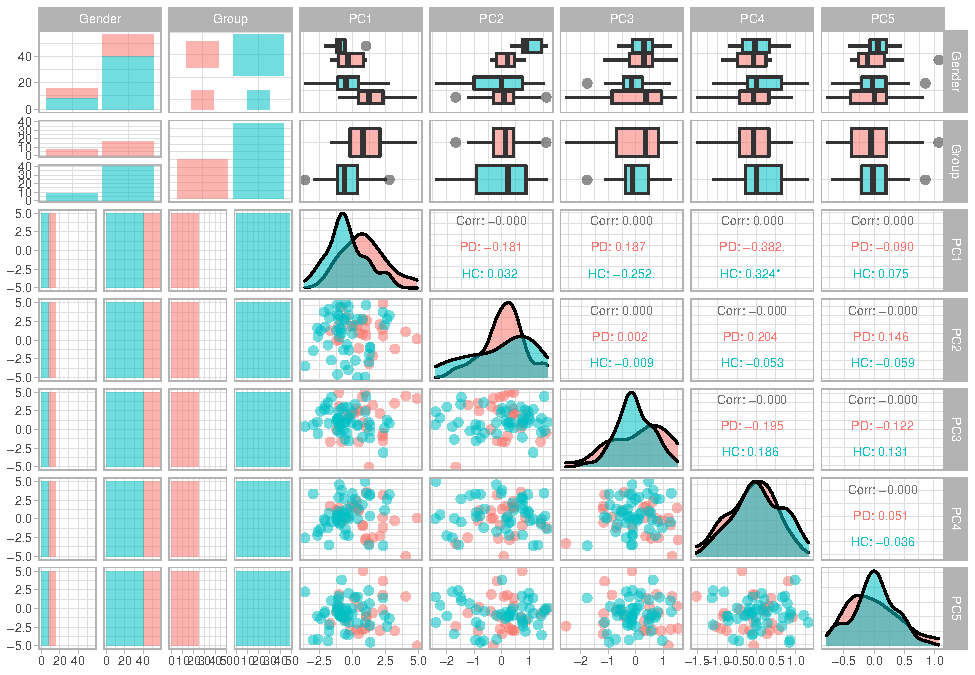
\includegraphics{dap_report_anja_probst_files/figure-latex/pca-ggpairs-1.pdf}
\caption{\label{fig:pca-ggpairs}ggpairs plot where the speech-related variables have been replaced by the principal components of a PCA.}
\end{figure}

\begin{longtable}[]{@{}
  >{\raggedright\arraybackslash}p{(\columnwidth - 2\tabcolsep) * \real{0.12}}
  >{\raggedright\arraybackslash}p{(\columnwidth - 2\tabcolsep) * \real{0.17}}@{}}
\caption{\label{tab:vif-after-pca} Variance inflation factors (vif) for the model based on
the PCA result (m.binom.pca).}\tabularnewline
\toprule
Term & VIF Value \\
\midrule
\endfirsthead
\toprule
Term & VIF Value \\
\midrule
\endhead
PC1 & 1.213 \\
Gender & 1.213 \\
\bottomrule
\end{longtable}

\clearpage

\hypertarget{diagnostic-plots-for-models}{%
\subsection{Diagnostic Plots for Models}\label{diagnostic-plots-for-models}}

Following are the diagnostic plots for the three logistic regression models described in the text.

\begin{figure}

{\centering 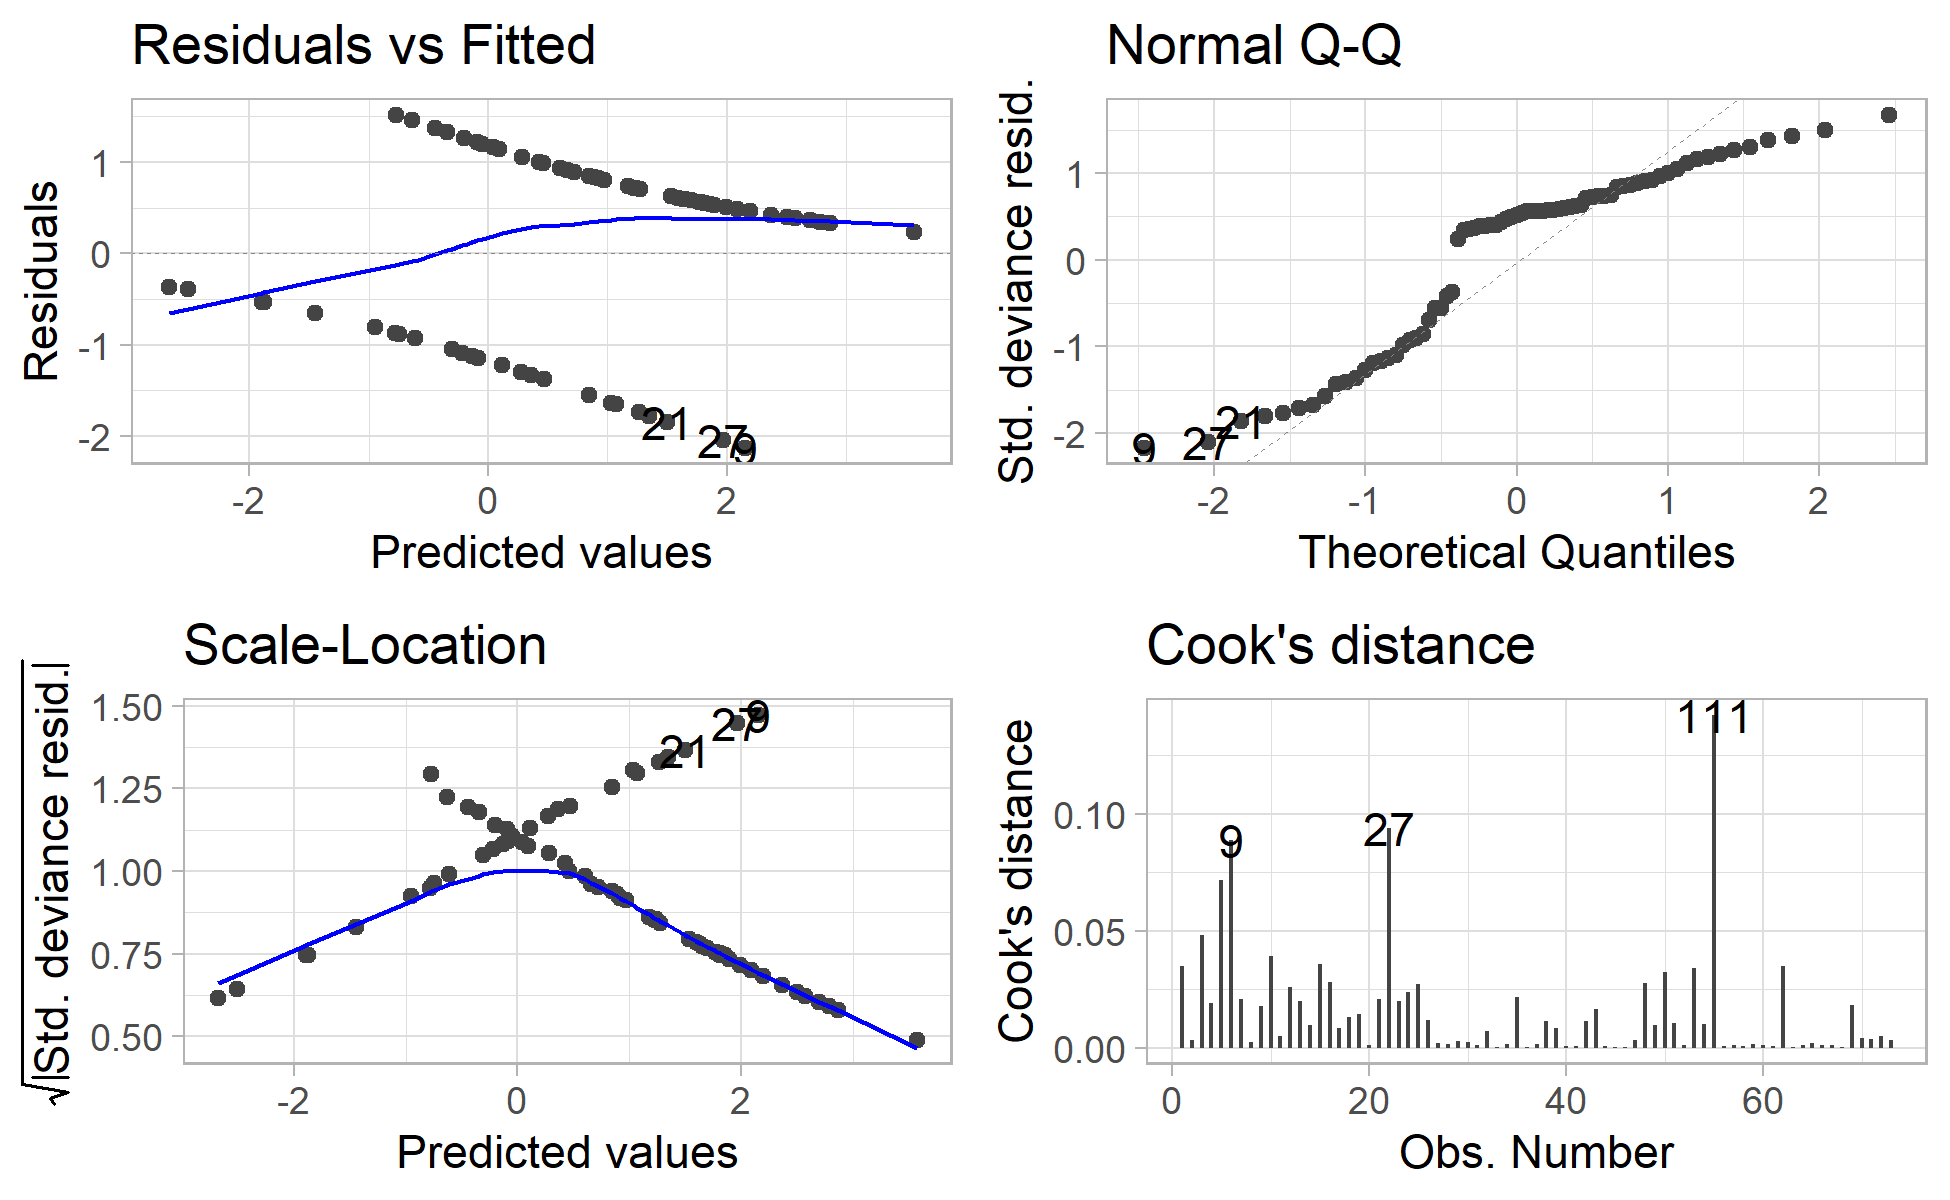
\includegraphics{dap_report_anja_probst_files/figure-latex/diagnostic-m.binom.no.interactions-1} 

}

\caption{Diagnostic plots for multiple logistic regression model (1) without interactions.}(\#fig:diagnostic-m.binom.no.interactions)
\end{figure}

\begin{figure}

{\centering 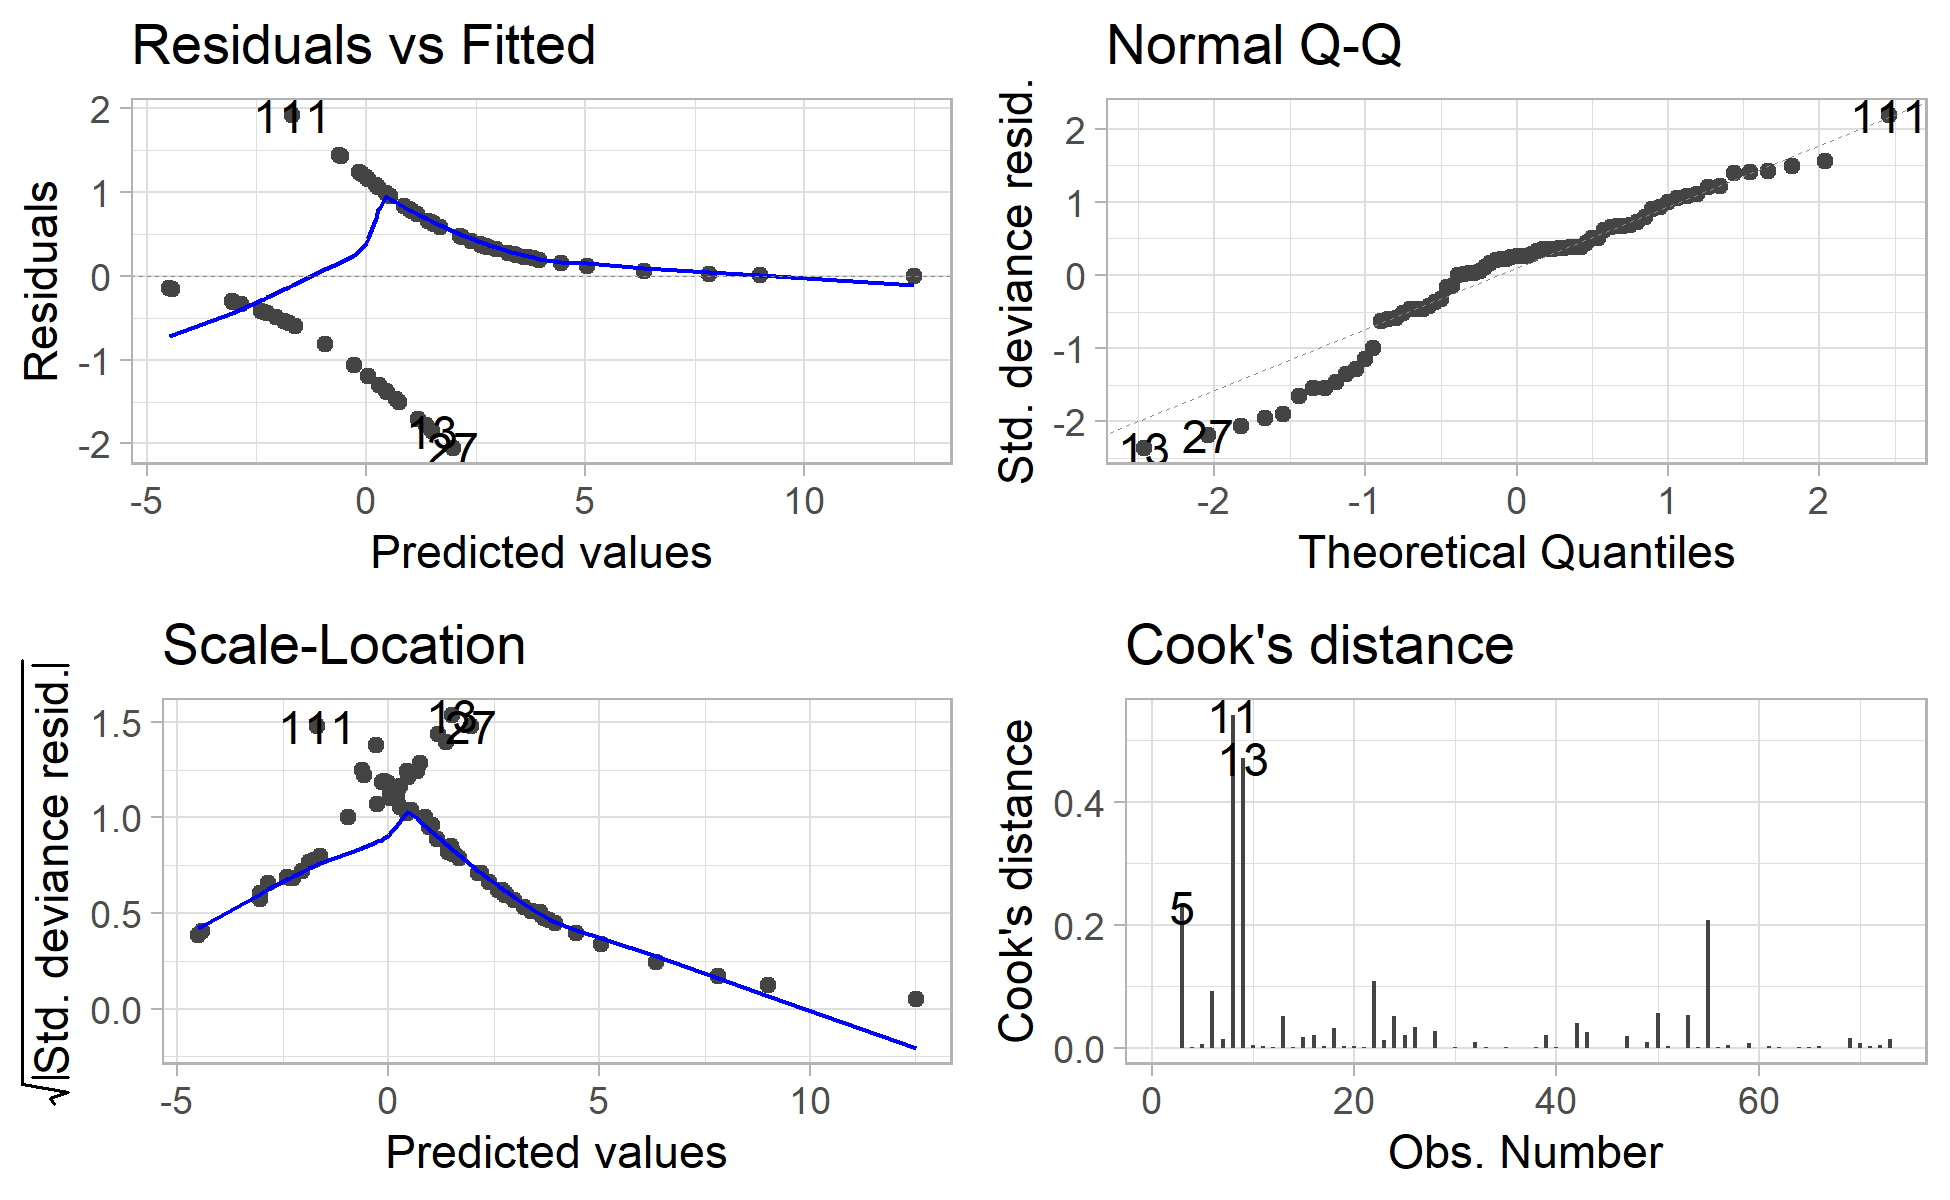
\includegraphics{dap_report_anja_probst_files/figure-latex/diagnostic-m.binom.interactions-1} 

}

\caption{Diagnostic plots for multiple logistic regression model (2) with interactions.}(\#fig:diagnostic-m.binom.interactions)
\end{figure}

\begin{figure}

{\centering 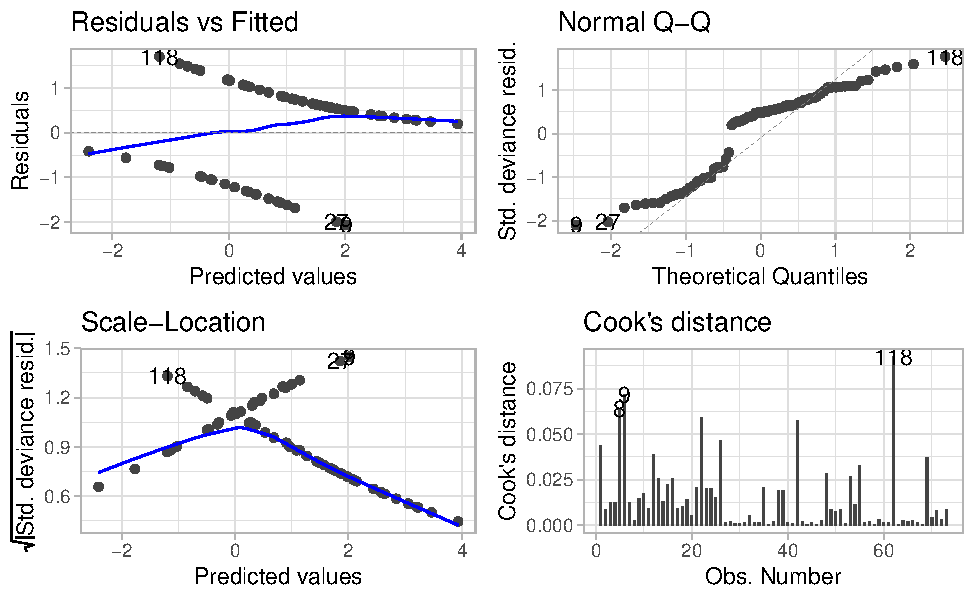
\includegraphics{dap_report_anja_probst_files/figure-latex/diagnostic-m.binom.pca-1} 

}

\caption{Diagnostic plots for multiple logistic regression model (3) after PCA.}(\#fig:diagnostic-m.binom.pca)
\end{figure}
\clearpage

\hypertarget{used-r-packages}{%
\section{Used R Packages}\label{used-r-packages}}

I used the following R packages during this project:
R (Version 4.1.1; R Core Team, 2021) and the R-packages \emph{apaTables} (Version 2.0.8; Stanley, 2021), \emph{bookdown} (Version 0.24; Xie, 2016), \emph{broom} (Version 0.7.10.9000; Robinson, Hayes, \& Couch, 2022), \emph{captioner} (Version 2.2.3; Alathea, 2015), \emph{car} (Version 3.0.12; Fox \& Weisberg, 2019; Fox, Weisberg, \& Price, 2020; Kuhn, 2021a), \emph{carData} (Version 3.0.4; Fox, Weisberg, \& Price, 2020), \emph{caret} (Version 6.0.90; Kuhn, 2021a), \emph{devtools} (Version 2.4.3; Wickham, Hester, Chang, \& Bryan, 2021), \emph{dials} (Version 0.0.10; Kuhn \& Frick, 2021), \emph{dplyr} (Version 1.0.7; Wickham, François, Henry, \& Müller, 2021), \emph{forcats} (Version 0.5.1; Wickham, 2021a), \emph{GGally} (Version 2.1.2; Schloerke et al., 2021), \emph{ggfortify} (Version 0.4.13; Tang, Horikoshi, \& Li, 2016), \emph{ggplot2} (Version 3.3.5; Wickham, 2016), \emph{ggpubr} (Version 0.4.0; Kassambara, 2020), \emph{gtsummary} (Version 1.5.0; Sjoberg, Whiting, Curry, Lavery, \& Larmarange, 2021), \emph{infer} (Version 1.0.0; Bray et al., 2021), \emph{kableExtra} (Version 1.3.4; Zhu, 2021), \emph{lattice} (Version 0.20.44; Sarkar, 2008), \emph{MASS} (Version 7.3.54; Venables \& Ripley, 2002a), \emph{modeldata} (Version 0.1.1; Kuhn, 2021b), \emph{MuMIn} (Version 1.43.17; Barton, 2020), \emph{nnet} (Version 7.3.16; Venables \& Ripley, 2002b), \emph{pacman} (Version 0.5.1; Rinker \& Kurkiewicz, 2018), \emph{pander} (Version 0.6.4; Daróczi \& Tsegelskyi, 2021), \emph{papaja} (Version 0.1.0.9997; Aust \& Barth, 2020), \emph{parsnip} (Version 0.1.7; Kuhn \& Vaughan, 2021a), \emph{patchwork} (Version 1.1.1; Pedersen, 2020), \emph{purrr} (Version 0.3.4; Henry \& Wickham, 2020), \emph{rcompanion} (Version 2.4.6; Mangiafico, 2021), \emph{readr} (Version 2.1.1; Wickham, Hester, \& Bryan, 2021), \emph{recipes} (Version 0.1.17; Kuhn \& Wickham, 2021), \emph{report} (Version 0.4.0; Makowski, Ben-Shachar, Patil, \& Lüdecke, 2021), \emph{reshape2} (Version 1.4.4; Wickham, 2007), \emph{rsample} (Version 0.1.1; Silge, Chow, Kuhn, \& Wickham, 2021), \emph{scales} (Version 1.1.1; Wickham \& Seidel, 2020), \emph{stargazer} (Version 5.2.2; Hlavac, 2018), \emph{stringr} (Version 1.4.0; Wickham, 2019), \emph{tibble} (Version 3.1.5; Müller \& Wickham, 2021), \emph{tidymodels} (Version 0.1.4; Kuhn \& Wickham, 2020), \emph{tidyr} (Version 1.1.4; Wickham, 2021b), \emph{tidyverse} (Version 1.3.1; Wickham et al., 2019), \emph{tinylabels} (Version 0.2.2; Barth, 2021), \emph{tune} (Version 0.1.6; Kuhn, 2021c), \emph{usethis} (Version 2.1.5; Wickham, Bryan, \& Barrett, 2021), \emph{vtable} (Version 1.3.3; Huntington-Klein, 2021), \emph{workflows} (Kuhn, 2021d; Version 0.2.4; Vaughan, 2021), \emph{workflowsets} (Version 0.1.0; Kuhn, 2021d), and \emph{yardstick} (Version 0.0.9; Kuhn \& Vaughan, 2021b)

\clearpage

\hypertarget{references}{%
\section*{References}\label{references}}
\addcontentsline{toc}{section}{References}

\hypertarget{refs}{}
\begin{CSLReferences}{1}{0}
\leavevmode\hypertarget{ref-R-captioner}{}%
Alathea, L. (2015). \emph{Captioner: Numbers figures and creates simple captions}. Retrieved from \url{https://CRAN.R-project.org/package=captioner}

\leavevmode\hypertarget{ref-R-papaja}{}%
Aust, F., \& Barth, M. (2020). \emph{{papaja}: {Prepare} reproducible {APA} journal articles with {R Markdown}}. Retrieved from \url{https://github.com/crsh/papaja}

\leavevmode\hypertarget{ref-R-tinylabels}{}%
Barth, M. (2021). \emph{{tinylabels}: Lightweight variable labels}. Retrieved from \url{https://cran.r-project.org/package=tinylabels}

\leavevmode\hypertarget{ref-R-MuMIn}{}%
Barton, K. (2020). \emph{MuMIn: Multi-model inference}. Retrieved from \url{https://CRAN.R-project.org/package=MuMIn}

\leavevmode\hypertarget{ref-R-infer}{}%
Bray, A., Ismay, C., Chasnovski, E., Couch, S., Baumer, B., \& Cetinkaya-Rundel, M. (2021). \emph{Infer: Tidy statistical inference}. Retrieved from \url{https://CRAN.R-project.org/package=infer}

\leavevmode\hypertarget{ref-R-pander}{}%
Daróczi, G., \& Tsegelskyi, R. (2021). \emph{Pander: An r 'pandoc' writer}. Retrieved from \url{https://CRAN.R-project.org/package=pander}

\leavevmode\hypertarget{ref-dashtipour2018speech}{}%
Dashtipour, K., Tafreshi, A., Lee, J., \& Crawley, B. (2018). Speech disorders in parkinson's disease: Pathophysiology, medical management and surgical approaches. \emph{Neurodegenerative Disease Management}, \emph{8}(5), 337--348.

\leavevmode\hypertarget{ref-R-car}{}%
Fox, J., \& Weisberg, S. (2019). \emph{An {R} companion to applied regression} (Third). Thousand Oaks {CA}: Sage. Retrieved from \url{https://socialsciences.mcmaster.ca/jfox/Books/Companion/}

\leavevmode\hypertarget{ref-R-carData}{}%
Fox, J., Weisberg, S., \& Price, B. (2020). \emph{carData: Companion to applied regression data sets}. Retrieved from \url{https://CRAN.R-project.org/package=carData}

\leavevmode\hypertarget{ref-R-purrr}{}%
Henry, L., \& Wickham, H. (2020). \emph{Purrr: Functional programming tools}. Retrieved from \url{https://CRAN.R-project.org/package=purrr}

\leavevmode\hypertarget{ref-R-stargazer}{}%
Hlavac, M. (2018). \emph{Stargazer: Well-formatted regression and summary statistics tables}. Bratislava, Slovakia: Central European Labour Studies Institute (CELSI). Retrieved from \url{https://CRAN.R-project.org/package=stargazer}

\leavevmode\hypertarget{ref-hlavnivcka2017automated}{}%
Hlavnička, J., Čmejla, R., Tykalová, T., Šonka, K., Ržička, E., \& Rusz, J. (2017). Automated analysis of connected speech reveals early biomarkers of parkinson's disease in patients with rapid eye movement sleep behaviour disorder. \emph{Scientific Reports}, \emph{7}(1), 1--13.

\leavevmode\hypertarget{ref-R-vtable}{}%
Huntington-Klein, N. (2021). \emph{Vtable: Variable table for variable documentation}. Retrieved from \url{https://CRAN.R-project.org/package=vtable}

\leavevmode\hypertarget{ref-R-ggpubr}{}%
Kassambara, A. (2020). \emph{Ggpubr: 'ggplot2' based publication ready plots}. Retrieved from \url{https://CRAN.R-project.org/package=ggpubr}

\leavevmode\hypertarget{ref-R-caret}{}%
Kuhn, M. (2021a). \emph{Caret: Classification and regression training}. Retrieved from \url{https://CRAN.R-project.org/package=caret}

\leavevmode\hypertarget{ref-R-modeldata}{}%
Kuhn, M. (2021b). \emph{Modeldata: Data sets used useful for modeling packages}. Retrieved from \url{https://CRAN.R-project.org/package=modeldata}

\leavevmode\hypertarget{ref-R-tune}{}%
Kuhn, M. (2021c). \emph{Tune: Tidy tuning tools}. Retrieved from \url{https://CRAN.R-project.org/package=tune}

\leavevmode\hypertarget{ref-R-workflowsets}{}%
Kuhn, M. (2021d). \emph{Workflowsets: Create a collection of 'tidymodels' workflows}. Retrieved from \url{https://CRAN.R-project.org/package=workflowsets}

\leavevmode\hypertarget{ref-R-dials}{}%
Kuhn, M., \& Frick, H. (2021). \emph{Dials: Tools for creating tuning parameter values}. Retrieved from \url{https://CRAN.R-project.org/package=dials}

\leavevmode\hypertarget{ref-R-parsnip}{}%
Kuhn, M., \& Vaughan, D. (2021a). \emph{Parsnip: A common API to modeling and analysis functions}. Retrieved from \url{https://CRAN.R-project.org/package=parsnip}

\leavevmode\hypertarget{ref-R-yardstick}{}%
Kuhn, M., \& Vaughan, D. (2021b). \emph{Yardstick: Tidy characterizations of model performance}. Retrieved from \url{https://CRAN.R-project.org/package=yardstick}

\leavevmode\hypertarget{ref-R-tidymodels}{}%
Kuhn, M., \& Wickham, H. (2020). \emph{Tidymodels: A collection of packages for modeling and machine learning using tidyverse principles.} Retrieved from \url{https://www.tidymodels.org}

\leavevmode\hypertarget{ref-R-recipes}{}%
Kuhn, M., \& Wickham, H. (2021). \emph{Recipes: Preprocessing and feature engineering steps for modeling}. Retrieved from \url{https://CRAN.R-project.org/package=recipes}

\leavevmode\hypertarget{ref-R-report}{}%
Makowski, D., Ben-Shachar, M. S., Patil, I., \& Lüdecke, D. (2021). Automated results reporting as a practical tool to improve reproducibility and methodological best practices adoption. \emph{CRAN}. Retrieved from \url{https://github.com/easystats/report}

\leavevmode\hypertarget{ref-R-rcompanion}{}%
Mangiafico, S. (2021). \emph{Rcompanion: Functions to support extension education program evaluation}. Retrieved from \url{https://CRAN.R-project.org/package=rcompanion}

\leavevmode\hypertarget{ref-R-tibble}{}%
Müller, K., \& Wickham, H. (2021). \emph{Tibble: Simple data frames}. Retrieved from \url{https://CRAN.R-project.org/package=tibble}

\leavevmode\hypertarget{ref-R-patchwork}{}%
Pedersen, T. L. (2020). \emph{Patchwork: The composer of plots}. Retrieved from \url{https://CRAN.R-project.org/package=patchwork}

\leavevmode\hypertarget{ref-R-base}{}%
R Core Team. (2021). \emph{R: A language and environment for statistical computing}. Vienna, Austria: R Foundation for Statistical Computing. Retrieved from \url{https://www.R-project.org/}

\leavevmode\hypertarget{ref-R-pacman}{}%
Rinker, T. W., \& Kurkiewicz, D. (2018). \emph{{pacman}: {P}ackage management for {R}}. Buffalo, New York. Retrieved from \url{http://github.com/trinker/pacman}

\leavevmode\hypertarget{ref-R-broom}{}%
Robinson, D., Hayes, A., \& Couch, S. (2022). \emph{Broom: Convert statistical objects into tidy tibbles}.

\leavevmode\hypertarget{ref-R-lattice}{}%
Sarkar, D. (2008). \emph{Lattice: Multivariate data visualization with r}. New York: Springer. Retrieved from \url{http://lmdvr.r-forge.r-project.org}

\leavevmode\hypertarget{ref-R-GGally}{}%
Schloerke, B., Cook, D., Larmarange, J., Briatte, F., Marbach, M., Thoen, E., \ldots{} Crowley, J. (2021). \emph{GGally: Extension to 'ggplot2'}. Retrieved from \url{https://CRAN.R-project.org/package=GGally}

\leavevmode\hypertarget{ref-R-rsample}{}%
Silge, J., Chow, F., Kuhn, M., \& Wickham, H. (2021). \emph{Rsample: General resampling infrastructure}. Retrieved from \url{https://CRAN.R-project.org/package=rsample}

\leavevmode\hypertarget{ref-R-gtsummary}{}%
Sjoberg, D. D., Whiting, K., Curry, M., Lavery, J. A., \& Larmarange, J. (2021). Reproducible summary tables with the gtsummary package. \emph{{The R Journal}}, \emph{13}, 570--580. \url{https://doi.org/10.32614/RJ-2021-053}

\leavevmode\hypertarget{ref-R-apaTables}{}%
Stanley, D. (2021). \emph{apaTables: Create american psychological association (APA) style tables}. Retrieved from \url{https://CRAN.R-project.org/package=apaTables}

\leavevmode\hypertarget{ref-R-ggfortify}{}%
Tang, Y., Horikoshi, M., \& Li, W. (2016). Ggfortify: Unified interface to visualize statistical result of popular r packages. \emph{The R Journal}, \emph{8}(2), 474--485. \url{https://doi.org/10.32614/RJ-2016-060}

\leavevmode\hypertarget{ref-R-workflows}{}%
Vaughan, D. (2021). \emph{Workflows: Modeling workflows}. Retrieved from \url{https://CRAN.R-project.org/package=workflows}

\leavevmode\hypertarget{ref-R-MASS}{}%
Venables, W. N., \& Ripley, B. D. (2002a). \emph{Modern applied statistics with s} (Fourth). New York: Springer. Retrieved from \url{https://www.stats.ox.ac.uk/pub/MASS4/}

\leavevmode\hypertarget{ref-R-nnet}{}%
Venables, W. N., \& Ripley, B. D. (2002b). \emph{Modern applied statistics with s} (Fourth). New York: Springer. Retrieved from \url{https://www.stats.ox.ac.uk/pub/MASS4/}

\leavevmode\hypertarget{ref-vos2016global}{}%
Vos, T., Allen, C., Arora, M., Barber, R. M., Bhutta, Z. A., Brown, A., \ldots{} others. (2016). Global, regional, and national incidence, prevalence, and years lived with disability for 310 diseases and injuries, 1990--2015: A systematic analysis for the global burden of disease study 2015. \emph{The Lancet}, \emph{388}(10053), 1545--1602.

\leavevmode\hypertarget{ref-R-reshape2}{}%
Wickham, H. (2007). Reshaping data with the {reshape} package. \emph{Journal of Statistical Software}, \emph{21}(12), 1--20. Retrieved from \url{http://www.jstatsoft.org/v21/i12/}

\leavevmode\hypertarget{ref-R-ggplot2}{}%
Wickham, H. (2016). \emph{ggplot2: Elegant graphics for data analysis}. Springer-Verlag New York. Retrieved from \url{https://ggplot2.tidyverse.org}

\leavevmode\hypertarget{ref-R-stringr}{}%
Wickham, H. (2019). \emph{Stringr: Simple, consistent wrappers for common string operations}. Retrieved from \url{https://CRAN.R-project.org/package=stringr}

\leavevmode\hypertarget{ref-R-forcats}{}%
Wickham, H. (2021a). \emph{Forcats: Tools for working with categorical variables (factors)}. Retrieved from \url{https://CRAN.R-project.org/package=forcats}

\leavevmode\hypertarget{ref-R-tidyr}{}%
Wickham, H. (2021b). \emph{Tidyr: Tidy messy data}. Retrieved from \url{https://CRAN.R-project.org/package=tidyr}

\leavevmode\hypertarget{ref-R-tidyverse}{}%
Wickham, H., Averick, M., Bryan, J., Chang, W., McGowan, L. D., François, R., \ldots{} Yutani, H. (2019). Welcome to the {tidyverse}. \emph{Journal of Open Source Software}, \emph{4}(43), 1686. \url{https://doi.org/10.21105/joss.01686}

\leavevmode\hypertarget{ref-R-usethis}{}%
Wickham, H., Bryan, J., \& Barrett, M. (2021). \emph{Usethis: Automate package and project setup}. Retrieved from \url{https://CRAN.R-project.org/package=usethis}

\leavevmode\hypertarget{ref-R-dplyr}{}%
Wickham, H., François, R., Henry, L., \& Müller, K. (2021). \emph{Dplyr: A grammar of data manipulation}. Retrieved from \url{https://CRAN.R-project.org/package=dplyr}

\leavevmode\hypertarget{ref-R-readr}{}%
Wickham, H., Hester, J., \& Bryan, J. (2021). \emph{Readr: Read rectangular text data}. Retrieved from \url{https://CRAN.R-project.org/package=readr}

\leavevmode\hypertarget{ref-R-devtools}{}%
Wickham, H., Hester, J., Chang, W., \& Bryan, J. (2021). \emph{Devtools: Tools to make developing r packages easier}. Retrieved from \url{https://CRAN.R-project.org/package=devtools}

\leavevmode\hypertarget{ref-R-scales}{}%
Wickham, H., \& Seidel, D. (2020). \emph{Scales: Scale functions for visualization}. Retrieved from \url{https://CRAN.R-project.org/package=scales}

\leavevmode\hypertarget{ref-wooten2004men}{}%
Wooten, G., Currie, L., Bovbjerg, V., Lee, J., \& Patrie, J. (2004). Are men at greater risk for parkinson's disease than women? \emph{Journal of Neurology, Neurosurgery \& Psychiatry}, \emph{75}(4), 637--639.

\leavevmode\hypertarget{ref-R-bookdown}{}%
Xie, Y. (2016). \emph{Bookdown: Authoring books and technical documents with {R} markdown}. Boca Raton, Florida: Chapman; Hall/CRC. Retrieved from \url{https://bookdown.org/yihui/bookdown}

\leavevmode\hypertarget{ref-R-kableExtra}{}%
Zhu, H. (2021). \emph{kableExtra: Construct complex table with 'kable' and pipe syntax}. Retrieved from \url{https://CRAN.R-project.org/package=kableExtra}

\end{CSLReferences}


\end{document}
